\documentclass[12pt]{report}

%Formattering

%Font og sprog
\usepackage[T1]{fontenc}
\usepackage[utf8]{inputenc}
\usepackage[danish]{babel}
\usepackage{caption}

%Page layout
\usepackage[a4paper,width=150mm,top=25mm,bottom=25mm, twoside]{geometry}
\usepackage{graphicx}
\usepackage{xcolor}
\usepackage{bm}
\usepackage{fancyhdr} %Header og footer, på alle normale sider
\pagestyle{fancy}
\fancyhead{}
\fancyhead[L]{\rightmark }
\fancyfoot{}
\fancyfoot[R]{\bfseries \thepage}
\fancyfoot[L]{\leftmark}
\renewcommand{\footrulewidth}{1pt}
\renewcommand{\chaptername}{Spørgsmål}
\usepackage{pgf,tikz}
\usepackage{mathrsfs}
\usetikzlibrary{arrows}

\usepackage[toc,page]{appendix}


%Diverse brugbare pakker

\usepackage{comment}
\usepackage{hyperref}
\usepackage{amssymb}
\usepackage{amsmath}
\usepackage{amsfonts}
\usepackage{framed}
\usepackage{etoolbox}
\usepackage{enumitem}
\usepackage{dsfont}
\usepackage[framed,amsmath,thmmarks]{ntheorem}
%Diverse Envirronments

\newtheorem{lemma}{Lemma}
\newtheorem{proposition}[lemma]{Proposition}
\newtheorem{theorem}[lemma]{Sætning}
\newtheorem{remark}[lemma]{Remark} 
\newtheorem{definition}[lemma]{Definition}
\theoremheaderfont{\normalfont\bfseries}
\theorembodyfont{\normalfont}
\theoremstyle{break}
\def\theoremframecommand{\colorbox[rgb]{1,.9,.9}}
\newshadedtheorem{eksempel}[lemma]{Eksempel}
\newenvironment{eks}[1]{%
		\begin{eksempel}[#1]
}{%
		\end{eksempel}
}
\newtheorem*{proof}{Bevis}
\newenvironment{pro}{\begin{bevis}}{\end{bevis}}
\AtEndEnvironment{proof}{$\null\hfill\blacksquare$}
\theoremstyle{break}
\newenvironment{AMS}{}{}
\newenvironment{keywords}{}{}
\newcommand{\by}{\mathbf{y}}
\newcommand{\bparam}{{\bm{\theta}}}
\newcommand{\bY}{\mathbf{Y}}
\newcommand{\bZ}{\mathbf{Z}}
\newcommand{\bparammax}{\widehat{\bparam}\left(\by\right)}
\newcommand{\bParammax}{\widehat{\bparam}\left(\bY\right)}
\newcommand{\like}{L\left(\by,\bparam\right)}
\newcommand{\E}[1]{\mathrm{E}\left[#1\right]}
\newcommand{\Var}[1]{\mathrm{Var}\left[#1\right]}
\newcommand{\Int}[1]{\int#1\,d\mu}
\newcommand{\Pois}{\text{Pois}}
\newcommand{\hatB}{\widehat{\bm{\beta}}}
\newcommand{\bmu}{\bm{\mu}}
\newcommand{\bbeta}{\bm{\beta}}
\newcommand{\RR}{\mathbb{R}}
\newcommand{\EE}{\mathbb{E}}
\newcommand{\FF}{\mathbb{F}}
\newcommand{\Q}{\mathcal{Q}}
\newcommand{\ts}{\tilde{\sigma}}
\newcommand{\FS}{\mathcal{S}}
\newcommand{\tps}{T_p\FS}
\newcommand{\G}{\mathcal{G}}
\newcommand{\DD}{\mathcal{D}}
\newcommand{\W}{\mathcal{W}}
\newcommand{\FI}{\mathcal{F}}
\newcommand{\PI}{\mathcal{P}}
\newcommand{\FII}{\mathcal{F}_{II}}
\newcommand{\FIU}{\underline{\mathcal{F}}}
\newcommand{\M}{\mathcal{M}^+}
\renewcommand{\L}{\mathcal{L}}
\newcommand{\K}{\mathbb{K}}
\newcommand{\D}{\mathbb{D}}
\newcommand{\GI}{\Gamma_{11}}
\newcommand{\GII}{\Gamma_{12}}
\newcommand{\GIII}{\Gamma_{22}}
\newcommand{\laengde}[1]{\lvert|#1\rvert|}
\newcommand{\1}{\mathds{1}}
\DeclareMathOperator{\tr}{trace}
\DeclareMathOperator{\inte}{int}
\DeclareMathOperator{\spa}{span}

\title{Dispositioner til mål- og integrationsteori, men også målteori og stokastiske processer}
\author{Mikkel Findinge}
\setcounter{chapter}{1}
\begin{document}
\maketitle
\definecolor{qqqqff}{rgb}{0.,0.,1.}
\definecolor{zzttqq}{rgb}{0.6,0.2,0.}

\section*{Notation og begrebsliste}
\renewcommand{\arraystretch}{3}
\begin{tabular}{p{0.3\linewidth}p{0.7\linewidth}}
Simpel funktion & Antager endeligt mange funktionsværdier.
\\
$\M=\M(X,\EE)$ & Mængden af $\EE$-målelige funktioner $f\colon X\to[0,\infty[$.
\\
Definition af $\int f\, d_\mu$ & $\sup\{\int s\, d\mu| s\in\M$, s simpel, $s\leq f\}$.
\\
$g$ er majorant for $\{f_n\}$ & $g\in\M(X,\EE),$ $\int g\, d\mu<\infty$, hvor $\lvert f_n\rvert\leq g, \forall n$.
\\
$f$ er $\mu-$integrabel & $f\colon X\to\RR, \EE-$målelig, $\int f^+\, d\mu<\infty$ og $\int f^-\, d\mu<\infty$.
\\
$\L(X,\EE,\mu)$ & Mængden af $\mu$-integrable funktioner.
\\
Fatous Lemma & $\{f_n\}\in\M\Rightarrow\int\left(\liminf\limits_nf_n\, d\mu\leq\right)\liminf\limits_n\int f_n\, d\mu.$
\\
$\K$ er fællesmængdestabilt & $A,B\in\K\Rightarrow A\cap B\in\K$.
\\
$\D(\K)$ & Den mindste $\sigma$-klasse, der indeholder $\K$.
\\
$\sigma(\K)$ & Den mindste $\sigma$-algebra, der indeholder $\K$.
\\
Frembringersystem & $\K$ er frembringersystem for $\EE$, hvis $\E = \sigma(\K)$.
\\
$(X,\EE,\mu)$ er $\sigma$-endelig & $X = \bigcup_{n = 1}^\infty  {A_n}$, hvor $A_n\in\EE$ med $\mu(A_n)<\infty$.
\\
$\L_p$ - p-dobbelt integrabel mht. $\mu$ & $\Int{|f|^p}<\infty$, hvor $f$ er $\EE$-målelig.
\\
$\laengde{f}_p$ & $\left(\Int{|f|^p}\right)^{1/p}$.
\\
$L_p(X,\EE,\mu)$ & Vektorrum, hvor $f\sim g\Leftrightarrow\laengde{f-g}_p=0$.
\end{tabular}


\newpage
%\addtocounter{chapter}{1}
\begin{comment}
	content...
\chapter*{Mål- og integrationsteori}
\section*{1. Monotonisætningen.}
\begin{theorem}
For enhver ikke-aftagende følge $f_1\leq f_2\leq\ldots$ af funktioner fra $\M$ gælder
\[\int(\lim f_n)d\mu = \lim\int f_n d\mu.\]
\end{theorem}
\begin{proof}
Bemærk først, at $f=\lim_nf_n =\sup_nf_n\in\M$, samt at $(\int f_n\, d\mu)_ {n=1,2\ldots}$ er stigende, så begge sider i ligningen har mening.

\bigskip

Da $f\geq f_n, \forall n\in\mathbb{N}$, er det klart, at 
\[\int f\, d\mu\geq\lim\limits_{n}\int f_n\, d\mu.\]
Den anden ulighed skal derfor blot vises. Ifølge definitionen af $\int f\, d\mu$ (se s. 1) kommer det ud på at vise, at 
\[\int s\, d\mu\leq\lim\limits_{n}\int f_n\, d\mu,\]
for en simpel, $\EE$-målelig funktion $s\colon X\to [0,\infty[$, hvor $s\leq f$. - Det vil være nok for et vilkårligt $a\in]0,1[$ at vise
\[a\int s\, d\mu = \int as\, d\mu\leq\lim\limits_{n}\int f_n\, d\mu.\]
Vi har, da $\forall x\in X$, hvor $0<f(x)$, så er $as(x)<f(x)=\lim_nf_n(x),$ og dermed $\exists n\in\mathbb{N}\colon as(x)<f_n(x)$. For $f(x)=0$, er $0=s(x)=f_1(x)=f_2(x)=\ldots$.

\bigskip

Sætter vi $E_n = \left\{ x \in X|as(x) \leqslant f_n(x) \right\},n = 1,2, \ldots,$ må $E_n$ for $n$ stort nok opfylde, at
\[\bigcup\limits_{n = 1}^\infty  {{E_n}}  = X.\]
Da $s$ og $f_n$ er $\EE$-målelige funktioner, tilhører $E_1\subseteq E_2\subset\ldots$ sigma-algebraen $\EE$ (Eksempel 2.15 i bog).

\bigskip

Definér afbildningen $E\mapsto\nu(E)=\int as1_E\, d\mu$. Vi kan sætte $s = \sum\nolimits_{i = 1}^n {{a_i}{1_{{A_i}}}}$, da $s$ er simpel. Da integralet af en sum af funktioner kan splittes op i flere integraler, samt konstanter kan tages uden for integraler fås
\[\nu (E) = \int {\sum\limits_{i = 1}^n {a{a_i}{1_{{A_i}}}} } d\mu  = \sum\limits_{i = 1}^n {a{a_i}\mu ({A_i} \cap E)}, \]
hvilket er et mål jvf. eksemplerne 3.2C og 3.2D. En egenskab for mål er, at $\mu(E_n)\nearrow\mu\left(\cup^{\infty}_{n=1}E_n\right)$, når $E_1\subseteq E_2\subset\ldots$, og dermed fås
\[\nu (E) = \int {as\cdot{1_{{E_n}}}} d\mu  \nearrow \nu (X) = \int {as\cdot{1_X}} d\mu  = \int {as} \,d\mu. \]
Da $as\cdot 1_{E_n}\leq f_n$ og dermed $\int as\cdot 1_{E_n}\, d\mu\leq\int f_n\, d\mu$ følger det ønskede
\[\int as\, d\mu = \lim\limits_{n}\int as\cdot 1_{E_n}\, d\mu\leq\lim\limits_{n}\int f_n\, d\mu.\]
\end{proof}
\newpage
%\addtocounter{chapter}{1}
\section*{2. Lebesgueintegral og integrabilitet.}
Beviser kun eksistens af målet.
\begin{theorem}
Der findes en afbildning $I_\mu\in\M(X,\EE)$ givet ved
\[I_\mu(s)=\Int{s}=\sum_{i=1}^{n}a_i\mu(A_i)\] for en simpel funktion $s$ med følgende egenskaber:
\begin{enumerate}
\item $I_\mu(1_E)=\mu(E)$ for $E\in\EE$.
\item $I_\mu(f+g)=I_\mu(f)+I_\mu(g)$ for $f,g\in\M$.
\item $\lim_{n\to\infty}I_\mu(f_n)=I_\mu(f)$ når $(f_n)\in\M$ er en følge så $f_n\nearrow f$.
\end{enumerate}
\end{theorem}
\begin{proof}
Bevis først de to lemma'er herunder.

\bigskip

Definéres for et vilkårligt $f\in\M$
\[\tilde{I}=\sup\left\{\Int{s}\vert s\in\M, s\text{ simpel},s\leq f\right\}\in[0,\infty].\]
Hvis $f\in\M$ selv er simpel indgår den i ovenstående, altså er $\tilde{I}(f)\geq\Int{f}$. Lemma 4 giver dog, at $\Int{f}\geq\Int{s}$, hvormed  $\tilde{I}(f)\leq \Int{f}$, og dermed er $\tilde{I}(f)=\Int{f} = I_\mu$. Altså har det mening at definere $I_\mu(f)=\Int{f}$ ved ovenstående for alle $f\in\M$.

\bigskip

Vi skal nu vise, at $I_\mu$ opfylder (1)-(3). (1) er en umiddelbar konsekvens af definitionen. (3) har sit eget eksamensspørgsmål, så det gennemgås ikke, men antages sandt. 

\bigskip

Vi kan finde følger $(s_n)$ og $(t_n)$ af simple funktioner fra $\M$, så $s_n\nearrow f$ og $t_n\nearrow g$, da $s_n+t_n\nearrow f+g$ giver (3) og Lemma 3, at
\begin{align*}
\Int{f+g}&=\lim\Int{s_n+t_n}=\lim\left(\Int{s_n}+\Int{t_n}\right) \\ & = \lim\Int{s_n}+\lim\Int{t_n}=\Int{f}+\Int{g}.
\end{align*}
\end{proof}
\begin{lemma}
For simple $\EE$-målelige funktioner $s,t\colon X\to[0,\infty[$ er $s+t$ $\EE$-målelig og \[\Int{s+t}=\Int{s}+\Int{t}.\]
\end{lemma}
\begin{proof}
Hvis $X=\bigcup_1^pC_h$, hvor $C_1,\ldots,C_p\in\EE$ er parvis disjunkte, og hvis $c_1,\ldots,c_p\in[0,\infty[$, da er
\[\Int{\sum_{h=1}^pc_h1_{C_h}} = \sum_{h=1}^pc_h\mu{C_h}.\]
Udelades tomme $C_h$, og erstattes led $c_{h_1}\mu(C_{h_1}),\ldots,c_{h_k}\mu(C_{h_k})$ på højre side med
\[c_{h_1}\sum_{i=1}^{k}\mu(c_{h_i})=c_{h_1}\mu(\bigcup_{i=1}^kC_{h_i}),\]
når $c_{h_1}=\ldots=c_{h_k}$, kommer vi tilbage til definitionen af \[\Int{\sum_{h=1}^pc_h1_{C_h}}.\]

\bigskip

Er $a_1,\ldots,a_m$ og $b_1,\ldots,b_m$ forskellige funktionsværdier for henholdsvis $s$ og $t$, og sættes $A_i = s^{-1}(\{a_i\}), i=1,\ldots,m$ og $B_j = t^{-1}(\{b_j\}), j=1,\ldots,n$, har vi
\[X = X\cap X = \left(\bigcup_{i=1}^m A_i\right)\cap\left(\bigcup_{j=1}^n B_j\right) = \bigcup_{i,j} (A_i\cap B_j),\]
hvor de $mn$ mængder $A_i\cap B_j\in\EE$ er parvis disjunkte. Da nu
\[s=\sum_{i,j}a_i1_{A_i\cap B_j},~~~~~~t=\sum_{i,j}b_j1_{A_i\cap B_j},\]
og dermed
\[s+t = s=\sum_{i,j}(a_i+b_j)1_{A_i\cap B_j},\]
hvoraf vi ser, at 
\[\Int{s}+\Int{t}=\sum_{i,j}a_i\mu(A_i\cap B_j)+\sum_{i,j}b_j\mu(A_i\cap B_j) = \sum_{i,j}(a_i+b_j)\mu(A_i\cap B_j)=\Int{s+t}.\]
\end{proof}
\begin{lemma}
For simple $\EE$-målelige funktioner $s,t\colon X\to[+,\infty[$, hvor $s\leq t$, gælder
\[\Int{s}\leq\Int{t}.\]
\end{lemma}
\begin{proof}
Da $t=s+(t-s)$ med $t-s\geq 0$ har vi
\[\Int{t}=\Int{s}+\Int{t-s}\geq\Int{s}.\]
\end{proof}


\newpage
%\addtocounter{chapter}{1}
\section*{3. Lebesgues Majorantsætning.}
\begin{theorem}
Lad $f_n\colon X\to\RR, n=1,2,\ldots,$ være $\EE$-målelige funktioner, og lad følgen $\{f_n(x)\}$ være konvergent i $\RR$ for alle $x\in X$. Hvis der eksisterer et $g\in\M(X,\EE)$ med $\int g\, d\mu<\infty$, sådan at $\forall n: \lvert f_n\rvert\leq g$, da er $f_n, \forall n$ og $f=\lim f_n$ alle integrable mht. $\mu$, og 
\begin{equation}\label{eq:3}
\int f_n \, d\mu \xrightarrow[n\to\infty]{}\int f\, d\mu.
\end{equation}
\end{theorem}
\begin{proof}
Lad majoranten $g$ være givet. Da $f_1, f_2,\ldots$ er $\EE$-målelige, så er $f= \lim f_n$ $\EE$-målelig. Desuden da $\lvert f_n\rvert\leq g$, og dermed $\lvert f\rvert\leq g$. Disse er derfor $\mu$-integrable.

\bigskip

\noindent Vi beviser nu \eqref{eq:3} i to trin. Først for $g(x)<\infty, \forall x\in X$, og dernæst inkluderer vi muligheden for, at $g(x)=\infty$ for nogle $x\in X$.

\bigskip

\noindent Da $\lvert f_n\rvert \leq g$, har vi, at $g+f_n\geq 0$ og $g-f_n\geq 0$. Da $\{f_n(x)\}$ er konvergent i $\RR$ for alle x, har vi, at
\[\liminf(g+f_n)=\lim(g+f_n)=g+f,\]
Men så giver Fatous lemma, at
\[\int (g+f) \, d\mu\leq\liminf\int(g+f_n)\,d\mu,\]
og dermed har vi
\begin{align*}
\Int{g}+\Int{f} & \leq\liminf\left(\Int{g}+\Int{f_n}\right) \\ & = \Int{g}+\liminf\Int{f_n}.
\end{align*}
Vi kan altså trække $\Int{g}$ fra på begge sider, og dermed opnås
\[\Int{f}\leq\liminf\Int{f_n}.\]
Tilsvarende for $g-f_n$ fås 
\[\Int{g-f}=\Int{g}-\Int{f},\]
hvilket giver
\begin{align*}
\Int{g}-\Int{f}&\leq\liminf\Int{g-f_n}\\&=\Int{g}-\limsup\Int{f_n},
\end{align*}
og så er
\[\limsup\Int{f_n}\leq\Int{f}.\]
Sammen holdt har vi
\[\Int{f}\leq\liminf\Int{f_n}\leq\limsup\Int{f_n}\leq\Int{f},\]
dermed er
\[\liminf\Int{f_n}=\limsup\Int{f_n}=\Int{f},\]
hvilket vil sige
\[\Int{f_n}\xrightarrow[n\to\infty]{}\Int{f}.\]

\bigskip

Vi gør det nu generelt ved at tillade, at $g(x)=\infty$ for nogle $x$. Lad $N=\{x\in X\vert g(x)=\infty\}$, så er $g\cdot 1_{X\backslash N}$ en $\mu$-integrabel majorant for $f_1\cdot 1_{X\backslash N}, f_2\cdot 1_{X\backslash N},\ldots,$ og dermed i følge ovenstående gælder
\[\Int{f_n\cdot 1_{X\backslash N}\xrightarrow[n\to\infty]{}\Int{f\cdot 1_{X\backslash N}}}.\]
Da $\infty 1_N\leq g$, og dermed \[\infty\mu(N) \leq \Int{f},\]
har vi, at $\Int{g}<\infty\Rightarrow\mu(N)=0$. Dette betyder altså, at
\[\Int{f_n}=\Int{f_n\cdot 1_{X\backslash N}}\text{ og }\Int{f}=\Int{f\cdot 1_{X\backslash N}}.\]
\end{proof}

\newpage
%\addtocounter{chapter}{1}
\section*{4. Entydighedssætningen for mål.}
\begin{definition}
Et system $\D$ af delmængder af en mængde $X$ kaldes en $\sigma$-klasse i $X$, hvis
\begin{enumerate}
\item $X\in\D$.
\item $\complement A\in\D$, hvis $A\in\D$.
\item $\bigcup_{n\in\mathbb{N}}A_n\in\D$, når $(A_n)_{n\geq 1}$ er en følge af parvist disjunkte mængder fra $\D$.
\end{enumerate}
\end{definition}
\begin{theorem}
Lad $\mu$ og $\nu$ være mål på en $\sigma$-algebra $\EE$ i $X$, og antag, at $\K$ er et fællesmængdestabilt frembringersystem for $\EE$.  Antag ydermere, at $X$ kan skrives som forening $\bigcup^\infty_nK_n$ med $K_1\subseteq K_2\subseteq\ldots$, hvor $K_n\in\K$ og $\mu(K_n)<\infty, n=1,2\ldots.$ Hvis $\mu(K)=\nu(K)$ for alle $K\in\K$, så er $\mu=\nu$.
\end{theorem}
\begin{proof}
Antag først, at $\forall K\in\K, \mu(K)=\nu(K)$, og sæt \[\D_n = \{E\in\EE\vert\mu(K_n\cap E)=\nu(K_n\cap E)\}, n=1,2,\ldots.\]
Det kommer nu ud på at vise, at $\D_n = \EE$, for $n=1,2,\ldots.$

\bigskip

\noindent Lad $K\in\K$. Da $\K$ er fællesmængdestabilt er $K_n\cap K\in\K$, og dermed $\mu(K_n\cap K)=\nu(K_n\cap K)$ for $n=1,2,\ldots$. Men så er $\K\subseteq\D_n$ for $n=1,2,\ldots$.

\bigskip

\noindent Vi vil nu vise, at $\D_n$ er en $\sigma$-klasse for $n=1,2,\ldots$.
\begin{enumerate}
\item Da $X=\bigcup_n K_n$, så er $X\in\D_n$. (Trivielt)
\item Lad $E\in\D_n$. Da $\mu(K_n)=\nu(K_n)<\infty$ er \[\mu ({K_n} \cap \complement E) = \mu ({K_n}) - \mu ({K_n} \cap E) = \nu ({K_n}) - \nu ({K_n} \cap E) = \nu ({K_n} \cap \complement E),\] og dermed er $\complement E\in\D_n$.
\item Lad $E_1, E_2,\ldots\in\D_n$ være parvist disjunkte, så er (jvf. definitionen af mål)
\[\mu ({K_n} \cap \bigcup\limits_j {{E_j}} ) = \sum\limits_j {\mu ({K_n} \cap {E_j})}  = \sum\limits_j {\nu ({K_n} \cap {E_j})}  = \nu ({K_n} \cap \bigcup\limits_j {{E_j}} ),\]
og dermed er $\bigcup_jE_j\in\D$.
\end{enumerate}
Men så må $\D(\K)\subseteq\D_n$. Lemma 5.3 i bogen siger, at hvis $\K$ er fællesmængdestabilt, da er $\D(\K)=\sigma(\K)$. Men da $\K$ er frembringersystem for $\EE$, så er $\D(\K)=\sigma(\K)=\EE$. Dermed er $D_n = \EE$ for $n=1,2,\ldots$, og dermed er 
\[\mu(K_n\cap E)=\nu(K_n\cap E), \forall E\in\EE, n\geq 1.\]
Da $K_1\cap E\subseteq K_2\cap E\subseteq\ldots$ og $\bigcap_n (K_n\cap E) = E$ får vi, at
\[\mu(E) = \lim_n\mu(K_n\cap E)=\lim_n\nu(K_n\cap E) = \nu(E), \forall E\in\EE.\]
\end{proof}

\newpage
%\addtocounter{chapter}{1}
\section*{5. Invarians af lebesguemålet; Målforhold.}
For billedmålet af $\mu$ under $\phi\colon(X,\EE)\to(Y,\FF)$ gælder
\[\phi(\mu)(B) = \mu(\phi^{-1}(B)),~~~~B\in\FF.\]
Ydermere siges et Borelmål at være invariant ved $\phi$, hvis $\phi(\mu)$ er lig med $\mu$, dvs.
\[\forall B\in\mathbb{B}_k\colon\mu(\phi^{-1}(B))=\mu(B).\]
(Husk: $\phi$ skal være en homeomorfi afbildning fra $\RR^k\to\RR^k$. Og Radonmål er et Borelmål (defineret på en Borelmængde), som har endelig værdi for enhver begrænset Borelmængde.)
\begin{theorem}
Lebesguemålet $m_k$ i $\RR^k$ er translationsinvariant.
\end{theorem}
\begin{proof}
Translationen $\tau_a$ for $a\in\RR^k$ defineret ved
\[\tau_a(x)=x+a,~~x\in\RR^k\]
er en homeomorf afbildning fra $\RR^k$ på sig selv med $\tau_a^{-1} = \tau_{-a}$. Ved translationen føres $m_k$ over i målet $\tau_a(m_k)$ og for hvert standardinterval $I$ i $\RR^k$ vil $\tau_a^{-1}(I) = \tau_{-a}(I)$ være et nyt standardinterval med samme kantlængder, hvorfor
\[\tau_a(m_k)(I)=m_k(\tau^{-1}(I))=m_k(I).\]
Entydighedssætningen giver da, at $\tau_a(m_k)=m_k$.
\end{proof}
\begin{theorem}
Lebesguemålet $m_k$ i $\RR^k$ er invariant ved enhver isometri $\phi\colon\RR^k\to\RR^k$ med hensyn til den euklidiske metrik.
\end{theorem}
\begin{proof}
Mængder $E,F\subset\RR^k$ kaldes kongruente, hvis der findes en isometri $\phi(E)=F$. Vi skal vise, at kongruente Borelmængder i $\RR^k$ har samme Lebesguemål. En isometri kan udtrykkes ved $\phi(x)=Ax+a$, hvor $A$ er en ortogonal matrix og $a\in\RR^k$.

\bigskip

Ved $\phi^{-1}$ føres $m_k$ over i Radonmålet $\nu=\phi^{-1}(m_k)$ defineret ved \[\nu(E)=m_k(\phi(E)),~~E\in\mathbb{B}_k.\]
Da vi nu har for $E\in\mathbb{B}_k$ og $a\in\RR^k$:
\[\nu(E+a)=m_k(\phi(E+a))=m_k(\phi(E)+\phi(a))=m_k(\phi(E))=\nu(E).\]
Altså er $\nu$ translationsinvariant, men i henhold til Sætning 5.16 er $cm_k$, for $0\leq c$, de eneste Radonmål i $\RR^k$, der har denne egenskab. Sættes
\[B=\{(x_1,\ldots,x_k)\vert\sum_{i=1}^kx_i^2<1\},\]
til enhedskuglen i $\RR^k$, er $\phi(B)=B$, da denne er invariant under en orthogonal afbildning. Dermed er
\[\nu(B)=m_k(\phi(B))=m_k(B), 0<m_k(B)<\infty,\]
hvormed $c=1$, altså $\nu=m_k$, dvs. $m_k$ er invariant ved $\phi^{-1}$.
\end{proof}

\newpage
%\addtocounter{chapter}{1}
\section*{6. Produktmål.}
\begin{theorem}
Lad $(X,\EE,\mu)$ og $(Y,\FF,\nu)$ være to $\sigma$-endelige målrum. Der findes et og kun et mål $\pi$ på produkt $\sigma$-algebraen $\EE\otimes\FF$ med egenskaben
\begin{equation}\label{produkt}
\pi(A\times B)=\mu(A)\nu(B), \text{ for } A\in\EE, B\in\FF.
\end{equation}
Målrummet $(X\times Y,\EE\otimes\FF,\mu\otimes\nu)$ er $\sigma$-endeligt.
\end{theorem}
\begin{proof}
{\bf{Entydighed:}} Entydighedssætningen for mål kræver, at vi har et stabilt frembringersystem, $\K$, for $\EE\otimes\FF$, og at $X\times Y = \bigcup_{n = 1}^\infty  {K_n}$ for $K_1\subseteq K_2\subseteq\ldots$.
Lader vi
\[\K = \{A\times B\vert A\in\EE,B\in\FF\},\]
er dette et fællesmængdestabilt frembringersystem for $\EE\otimes\FF$, da
\[\left(A_1\times B_1\right)\cap\left(A_2\times B_2\right) = \left(A_1\cap A_2\right)\times\left(B_1\cap B_2\right).\]
$\sigma$-endeligheden giver, at der findes $A_1\subseteq A_2\subseteq\ldots\in\EE$ og $B_1\subseteq B_2\subseteq\ldots\in\FF$ med $\mu(A_n)<\infty$ og $\nu(B_n)\infty$, sådan at $X = \bigcup_{n = 1}^\infty  {A_n}$ og $Y=\bigcup_{n=1}^\infty {B_n}$. Lader vi $K_n=A_n\times B_n, n=1,2\ldots$ gælder $K_1\subseteq K_2\subseteq\ldots\in\K$, og $X\times Y=\bigcup_{n=1}^\infty K_n$. Hvis $\pi$ og $\rho$ er mål på $\EE\otimes\FF$, som opfylder \eqref{produkt}, er
\[\pi(A\times B)=\mu(A)\nu(B)=\rho(A\times B), \text{ for }A\in\EE,B\in\FF,\]
og $\mu(K_n)=\mu(A)\nu(B)<\infty.$ Dermed giver entydighedssætningen for mål, at $\pi=\rho$. Ydermere ses det, at $(X\times Y,\EE\otimes\FF,\pi)$ er $\sigma$-endeligt.

\bigskip 

\noindent{\bf{Eksistens:}} Lad $\pi\colon\EE\otimes\FF\to[0,\infty]$ være givet ved
\[\pi(G)=\int_X\nu(G_x)\,d\mu(x).\]
Vi skal først vise, at integralet giver mening ved at vise, at $x\mapsto\nu(G_x)$ er $\EE$-målelig og dernæst vise, at $\pi(G)$ er et mål, samt er lig \eqref{produkt}. Vi starter med $\EE-$måleligheden:
\begin{lemma}
For alle $G\in\EE\otimes\FF$ er $\phi_G\colon X\to[0,\infty]$ defineret ved $\phi_G(x)=\nu(G_x)$ en $\EE$-målelig funktion.
\end{lemma}
\begin{proof}
Sætning 6.3 i bogen giver, at $G_x\in\FF$, og dermed giver $\phi_G$ mening. $\phi_G$ har bl.a. egenskaberne:
\begin{enumerate}[label=(\alph*)]
\item For $G=A\times B$ med $A\in\EE, B\in\FF$ gælder $\phi_G = \nu(B)1_A$.
\item Hvis $G_1,G_2,\ldots\in\EE\otimes\FF$ er parvis disjunkte, og $G=\bigcup_1^\infty G_n$, da er \[\phi_G = \sum\limits_1^\infty\phi_{G_n}.\] 
\end{enumerate}
Vi viser første del af Lemma'et under forudsætning af $\nu(Y)<\infty$.

\bigskip

Grundet (a) har vi, at 
\[\K\subseteq\{G\in\EE\otimes\FF\vert\phi_G\in\M(X,\EE)\}=\D.\]
Da $\K\subseteq\D$ er $X\times Y\in\D$.\\
Hvis $G_1,G_2,\ldots\in\D$ er parvis disjunkte, så er $\phi_{G_n}\in\M(X,\EE)$, men så giver regler for grænser, at $\sum_1^\infty\phi_{G_n}\in\M(X,\EE)$, hvilket af (b) er $\phi_G$. Dermed er $G=\bigcup_1^\infty G_n\in\D$.\\
Da $\phi_{X\times Y} = \phi_G + \phi_{\complement G}$ og antaget, at  $\phi_{X\times Y}(x)=\nu(Y)<\infty$, har vi, at $\phi_G$ antager endelige værdier - dermed er $\phi_{\complement G} = \nu(Y)-\phi_G\in\M(X,\EE)$, hvormed $\complement G\in\D$.\\
Altså er $\D$ en $\sigma$-klasse. Da $\K$ er et fællesmængdestabilt frembringersystem for $\EE\otimes\FF$ giver Fundamentallemmaet, at $\D(\K)=\sigma(\K)=\EE\otimes\FF$, men da $\D$ er en $\sigma$-klasse indeholdende $\K$ er $\D(\K)\subseteq\D$, men så er $\D=\EE\otimes\FF$.

\bigskip

\footnote{Spring sidste del af lemmaet over, hvis for meget tid bruges.}For det generelle tilfælde bruges $\sigma$-endeligheden for $(Y,\FF,\nu)$, da vi dermed har $B_1\subseteq B_2\subseteq\ldots\in\FF$ med $\nu(B_n)<\infty, Y=\bigcup_1^\infty B_n$. For fast $n$ betragtes målet $\nu_n\colon\FF\to[0,\infty]$ defineret ved $\nu_n(B)=\nu(B\cap B_n)$. Da $\nu_n(Y)=\nu(B_n)<\infty$, kan vi af første del konkludere, at
\[x\mapsto\phi^{(n)}_G(x)=\nu(G_x)\in\M(X,\EE).\]
En egenskab for mål giver os da, at 
\[\phi^{(n)}_G(x)=\nu(G_x\cap B_n)\nearrow\nu(G_x)=\phi_G(x),\]
og dermed vil grænsefunktionen $\phi_G\in\M(X,\EE).$
\end{proof}
Nu har vi vist, at integralet før lemmaet har mening, og nu skal det blot vises, at $\pi\colon\EE\otimes\FF\to[0,\infty]$ er et mål, der opfylder \eqref{produkt}.\\
Hvis $G_1,G_2,\ldots\in\EE\otimes\FF$ er parvis disjunkte, og $G=\bigcup_1^\infty G_n$, da er $\phi_G=\sum_1^\infty\phi_{G_n}$ i følge (b), og med sætningen, der kan bytte integral og sum, har vi:
\[\pi(G)=\Int{\phi_G}=\sum\limits^\infty_1\Int{\phi_{G_n}}=\sum\limits^\infty_1\pi(G_n).\]
For $G=A\times B$ med $A\in\EE, B\in\FF$ finder vi ifølge (a), at
\[\pi(A\times B)=\Int{\nu(B)1_A}=\nu(B)\Int{1_A}=\nu(B)\mu(A).\]
Men så stemmer integralet overens med \eqref{produkt}, og vi har specielt, at $G=\emptyset=\emptyset\times\emptyset\Rightarrow\pi(\emptyset)=0$.
\end{proof}

\newpage
%\addtocounter{chapter}{1}
\section*{7. Tonelli og Fubinis sætninger.}
\begin{theorem}[Tonellis sætning]
Lad $(X,\EE,\mu)$ og $(Y,\FF,\nu)$ være $\sigma$-endelige målrum. For $f\in\M(X\times Y,\EE\otimes\FF)$ gælder
\begin{enumerate}
\item funktionen $x\mapsto\int_Yf_x\,d\nu = \int_Yf(x,y)\nu(y)$ tilhører $\M(X,\EE)$.
\item $\int_{X\times Y}f\,d(\mu\otimes\nu)=\int_X(\int_Yf(x,y)\,d\nu(y))\,d\mu(x)$.
\end{enumerate}
\end{theorem}
\begin{proof}
For $f\in\M(X\times Y,\EE\otimes\FF)$ med $x\in X$ vil $f_x\in\M(Y,\FF)$ (Sætning 6.3). Vi definerer $g\colon X\to[0,\infty]$ ved $g(x)=\int f_x\,d\nu$. Dermed siger (1), at $g\in\M(X,\EE)$, og (2) siger $\int f\,d\mu\otimes\nu=\Int{g}$.

\bigskip

Beviset køres i 3 trin. Første er for indikatorfunktionen, dernæst for simple funktioner og sidst udvides til vilkårlige funktioner.

\bigskip

{\textbf{Indikatorfunktionen}} $f=1_G$ på $X\times Y$ med $G\in\EE\otimes\FF$ har for ethvert $x\in X$, at $(1_G)_x=1_{G_x}$. Lemma 6.7 siger, at funktionen
\[x\mapsto\nu(G_x)=\int(1_G)_x\,d\nu\]
tilhører $\M(X,\EE)$, og Korollar 6.8 giver, at dens $\mu$-integral er $\mu\otimes\nu(G)=\int 1_G\,d\mu\otimes\nu.$

\bigskip

{\textbf{Simple funktioner}} på formen $f=\sum_{j=1}^na_j1_{G_j}$ på $X\times Y$ med $0<a_j<\infty, G_j\in\EE\otimes\FF$. Dette følger af indikatorfunktionerne - blot vis, at summen af to indikatorfunktioner samt en konstant ganget på en indikatorfunktion giver .

\bigskip

{\textbf{En vilkårlig funktion}} $f\in\M(X\times Y,\EE\otimes\FF)$ kan fås som grænsefunktion for en følge $f_1\leq f_2\leq\ldots$ af simple $\EE\otimes\FF$-målelige funktioner $f_n\colon X\times Y\to[0,\infty[$ (Sætning 4.1). Lebesgues monotonisætning giver, at 
\[\int_{X\times Y}f\,d(\mu\otimes\nu)=\lim\limits_{n\to\infty}\int_{X\times Y}f_n\,d(\mu\otimes\nu).\]
For hvert $x\in X$ har vi $(f_n)_x\nearrow f_x$ og dermed
\[g_n(x)=\int_Y(f_n)_x\,d\nu\nearrow g(x)=\int_Y f_x\,d\nu\]
ifølge Lebesgues monotonisætning. Da nu $g_n\in\M(X,\EE)$ og $g_n\nearrow g$, er $g\in\M(X,\EE)$, samt
\[\int_X g\,d\mu = \lim\limits_{n\to\infty}\int_Xg_n\,d\mu\]
ifølge lebesgues monotonisætning. Da $\int_{X\times Y}f\,d(\mu\otimes\nu)=\int_Xg_n\,d\mu, n=1,2,\ldots,$ sluttes endelig
\[\int_{X\times Y}f\,d(\mu\otimes\nu)=\int_X g\,d\mu.\]
\end{proof}


\newpage
%\addtocounter{chapter}{1}
\section*{8. Hölders og Minkowskis uligheder.}
\begin{theorem}[Minkowskis ulighed]
Når $f,g\in\L_p(X,\EE,\mu)$, hvor $1\leq p<\infty$, da er $f+g\in\L_p(X,\EE,\mu)$ og \[\laengde{f+g}_p\leq\laengde{f}_p+\laengde{g}_p.\]
\end{theorem}
\begin{proof}
Da $f+g$ er $\EE$-målelig, og 
\[\Int{|f+g|^p}\leq\Int{(|f|+|g|)^p}\leq 2^p\Int{|f|^p}+2^p\Int{|g|^p}<\infty,\]
er $f+g\in\L(X,\EE,\mu)$.

\bigskip

Vi antager, at $p>1$, og lader $q$ være givet ved $p^{-1}+q^{-1}=1$. Betragt
\[\laengde{f+g}_p^p=\Int{|f+g|^p}=\Int{|f+g||f+g|^{p-1}}\leq\Int{|f||f+g|^{p-1}}+\Int{|g||f+g|^{p-1}}.\]
Idet $f+g\in\L_p$, er funktionen $|f+g|^{p-1}$  $\EE$-målelig, og 
\[\Int{|f+g|^{(p-1)q}}=\Int{|f+g|^p}<\infty,\]
da $pq = p+q$, og dermed er $|f+g|^{p-1}\in\L_q$ med
\[\laengde{|f+g|^{p-1}}_q=\left(\Int{|f+g|^{(p-1)q}}\right)^{1/q}=\left(\Int{|f+g|^p}\right)^{1/q} = \laengde{f+g}_p^{p/q}=\laengde{f+g}_p^{p-1}.\]
Hölders ulighed giver så
\[\Int{|f||f+g|^{p-1}}\leq\laengde{f}_p\laengde{f+g}_p^{p-1},\]
\[\Int{|g||f+g|^{p-1}}\leq\laengde{g}_p\laengde{f+g}_p^{p-1}.\]
Sammenholdt har vi altså
\[\laengde{f+g}_p^p\leq(\laengde{f}_p+\laengde{g}_p)\laengde{f+g}_p^{p-1},\]
og ganges begge sider med $\laengde{f+g}^{1-p}_p$ opnås Minkowskis ulighed.
\end{proof}


\newpage
%\addtocounter{chapter}{1}
\section*{9. Lebesguerummene $L_p$ og deres fuldstændighed.}
Lebesguerummene, $L_p$, har samlet funktioner fra $\L_p$ i klasser ved ækvivalensrelationen \[f\sim g\Leftrightarrow\laengde{f-g}_p=0.\]
\begin{theorem}
Lad $(X,\EE,\mu)$ være et målrum og $1\leq p<\infty$. Funktionsrummet $\L_p=\L_p(X,\EE,\mu)$ er fuldstændigt. (Eller Lebesguerummet $L_p$ er et Banachrum jvf. Sætning 7.17).
\end{theorem}
\begin{proof}
Vi ved, at $L_p$ er et vektorrum med seminorm \[\laengde{f}_p=\left(\Int{|f|^p}\right)^{1/p}, f\in\L_p(X,\EE,\mu).\] Dermed er det nok at vise, at  $\sum_1^\infty g_k$ med $g_k\in\L_p$, hvor $\sum_1^\infty \laengde{g_k}_p < \infty$, er konvergent i $\L_p$ jvf. Sætning 7.16. Vi søger altså en funktion $f\in\L_p$, sådan at \[\laengde{f-\sum\limits_{k=1}^ng_k}_p\to 0,\, for\,\,n\to\infty.\]

\bigskip

Lad \[h(x)=\sum\limits_{k=1}^\infty|g_k(x)|,~~x\in X.\]
For hvert $x\in X$ sådan at $h(x)<\infty$ er $h\colon X\to[0,\infty]$ $\EE$-målelig, og $\sum_1^\infty g_k$ er absolut konvergent.

\bigskip

For $n\to\infty$ er $\sum_1^n|g_k(x)|\nearrow h(x)$ for alle $x\in X$, og dermed
\[\left(\sum\limits_{k=1}^n|g_k|\right)^p\nearrow (h(x))^p.\]
Lebesgues monotonisætning giver nu
\[\Int{\left(\sum\limits_{k=1}^n|g_k|\right)^p}\nearrow\Int{h^p},\]
hvormed vi kan opnå
\[\laengde{\sum\limits_{k=1}^n|g_k|}_p\nearrow\left(\Int{h^p}\right)^{1/p}.\]
Af Minkowskis ulighed har vi, at $\laengde{\sum_1^n|g_k|}_p\leq\sum_1^n\laengde{g_k}_p$ for alle $n\in\mathbb{N}$, og derfor er
\[\left(\Int{h^p}\right)^{1/p}\leq \sum\limits_{k=1}^n\laengde{g_k}_p<\infty.\]
Men så er $\Int{h^p}<\infty$, og dermed giver Korollar 4.5, at 
\[N=\{x\vert h(x)=\infty\}=\{x\vert (h(x))^p=\infty\}\]
har mål $\mu(N)=0$. Rækken $\sum_1^\infty g_k(x)$ er altså absolut konvergent f or $\mu$-næsten alle $x\in X$, og dermed kan vi definere $f\colon X\to\mathbb{C}$ ved
\[f\left( x \right) = \left\{ \begin{gathered}
  \sum_{k=1}^\infty g_k(x) \hfill ~~for\,\, x\in X\backslash N \\
  0~~for\,\, x\in N. \hfill \\ 
\end{gathered}  \right.\]
Af Tuborg-resultatet og grænseværdi-sætninger er $f$ målelig. Derudover er $|f(x)\leq h(x), x\in X$, hvoraf
\[\laengde{f}_p=\left(\Int{|f|^p}\right)^{1/p}\leq\left(\Int{h^p}\right)^{1/p}\leq\sum\limits_{k=1}^n\laengde{g_k}_p<\infty.\]
Dermed er $f\in\L_p$. Da $\sum_1^n\to f$ $\mu$-n.o, og $h$ er en majorant giver Sætning 7.10, at $\laengde{f-\sum_1^n g_k}_p\to 0$, for $n\to\infty$.
\end{proof}

\bigskip

Ekstra detalje: $\laengde{\cdot}_p$ er ikke en almindelig norm i $\L_p(X,\EE,\mu)$, da
\[\laengde{f}_p=\left(\Int{|f|^p}\right)^{1/p} = 0\Leftrightarrow f=0\,\,\mu-n.o.\]


\newpage
%\addtocounter{chapter}{1}
\section*{10. Fouriertransformationen på $\RR^k$.}
\begin{definition}
Når $f\colon\RR^k\to\mathbb{C}$ tilhører $\L_1(\RR)$, defineres den Fourier-transformerede af $f$, $\hat{f}\colon\RR^k\to\mathbb{C}$, ved 
\[\hat{f}(\xi) = \int_{\RR^k}e^{-i\xi\cdot x}f(x)\,dx,~~for\,\,\xi\in\RR^k.\]
Afbildningen $\FI\colon f\mapsto\hat{f}$ kaldes Fourier-transformationen.
\end{definition}
\begin{theorem}
Fouriertransformationen $\FI$ er en kontinuert lineær afbildning af $L_1(\RR^k)$ ind i $C_b(\RR^k)$, og der gælder
\[\laengde{\hat{f}}_u\leq\laengde{f}_1~~~~for~~f\in\L_1(\RR^k).\]
\end{theorem}
\begin{proof}

\end{proof}

\begin{theorem}
Lad $f\in\L_1(\RR)$ og $\xi\in\RR$.
\begin{enumerate}
\item Hvis $xf(x)\in\L_1(\RR)$, så er $\hat{f}\in C^1(\RR)$ og \[\FI(xf(x))(\xi)=i\hat{f}^\prime(\xi).\]
\item Hvis $f\in C^1(\RR)$ og $f^\prime\in\L_1(\RR)$ så er \[\FI(f^\prime)(\xi)=i\xi\hat{f}(\xi).\]
\end{enumerate}
\begin{proof}
For (1) giver Sætning 4.28, at \[\hat{f}^\prime(\xi)=\int\frac{\partial}{\partial\xi}\left(e^{-i\xi x}f(x)\right)\,dx=\int -ixe^{-i\xi x}f(x)\,dx=-i\FI(xf(x))(\xi),\]
da $g=|xf(x)|$ er en majorant for $x\mapsto-ixe^{-i\xi x}f(x),~~\xi\in\RR$.

\bigskip

For (2) bruger vi, at $\int_{|x|\geq n}|f^\prime(t)|\, dt\to 0,$ for $n\to\infty$ ifølge Lebesgues monotonisætning. For ethvert $\epsilon$ findes altså et $N\in\mathbb{N}$, så
\[\int_{|x|\geq N}|f^\prime(t)|\, dt\leq\epsilon,\]
hvoraf $x_1,x_2\geq N$ eller $x_1,x_2\leq-N$, og dermed
\[|f(x_2)-f(x-1)|=\lvert\int_{x_1}^{x_2}f^\prime(t)\,dt\rvert\leq\int_{|x|\geq N}|f^\prime(t)|\, dt\leq\epsilon,\]
hvoraf vi ser, at $\lim_{x\to\pm\infty}f(x)$ eksisterer.

\bigskip

Lad $\lim_{x\to\infty}f(x)=a\neq 0$, så findes $N>0$ så $|f(x)|\geq\frac{1}{2}|a|$ for $x\geq N$, hvilket strider mod, at $f$ er integrabel. På samme måde ses $\lim_{x\to-\infty}f(x)=0$. For $x_1<x_2$ giver partiel integration
\[\int_{x_1}^{x_2}e^{-i\xi x}f^\prime(x)\,dx=[e^{-i\xi x}f(x)]_{x_1}^{x_2}+i\xi\int_{x_1}^{x_2}e^{-i\xi x}f(x)\,dx.\]
Lad vi $x_1\to-\infty$ og $x_2\to\infty$ vil $f(x)\to 0$, og integralerne bliver til
\[\FI(f^\prime)(\xi)=i\xi\hat{f}(\xi),\]
da $f,f^\prime\L_1(\RR)$ pr. antagelse.
\end{proof}
\end{theorem}

\newpage
%\addtocounter{chapter}{1}
\section*{11. Foldning på $\RR^k$.}
\begin{definition}
Ved foldningen $f\ast g$ af to Borelfunktioner $f,g\colon\RR^k\to\mathbb{C}$ forstås funktionen \[f\ast g(x)=\int_{\RR^k}f(x-t)g(t)\,dt,~~~x\in\RR^k,\]
hvis definitionsområde er mængden 
\[\DD(f\ast g) = \left\{x\in\RR^k\vert\int|f(x-t)g(t)|\,dt<\infty\right\}.\]
\end{definition}
\begin{theorem}
For $f,g\in\L_1(\RR^k)$ er foldningen defineret for næsten alle $x\in\RR^k$ og bestemmer et element i $L_1(\RR^k)$, som betegnes $f\ast g$ for hvilket, der gælder \[\laengde{f\ast g}_1\leq\laengde{f}_1\laengde{g}_1.\]
\end{theorem}
\begin{proof}
Da $f\otimes g$ af Lemma 6.2 er Borelmålelig på $\RR^{2k}$ gælder dette også for sammensætningen $(x,t)\mapsto(x-t,t)$, dvs.
\[(x,t)\mapsto f(x-t)g(t),~~~~x,t\in\RR^k.\]
Denne funktion tilhører $\L_1(\RR^{2k})$, da vi med Tonellis sætning og translationsinvariansen af Lebesguemålet i $\RR^k$ finder
\begin{align*}
\int_{\RR^{2k}}|f(x-t)g(t)\,d(x,t) & =\int_{\RR^k}\left(|g(t)|\int_{\RR^k}|f(x-t)|\,dx\right)\,dt \\ &=\int_{\RR^k}\left(|g(t)|\int_{\RR^k}|f(x)|\,dx\right)\,dt = \laengde{f}_1\laengde{g}_1<\infty.
\end{align*}
Fubinis sætning giver nu, at $t\mapsto f(x-t)g(t)$ er integrabel for næsten alle $x\in\RR^k$, og at den næsten overalt i $\RR^k$ definerede funktion $f\ast g$ bestemmer et element i $L_1(\RR^k)$.

\bigskip

Da
\[|(f\ast g)(x)|\leq\int_{\RR^k}|f(x-t)g(t)|\,dt\]
får vi ved at tage integralet på begge sider:
\[\laengde{f\ast g}_1\leq\int_{\RR^k}\int_{\RR^k}|f(x-t)g(t)\,dtdx=\int_{\RR^{2k}}|f(x-t)g(t)\,d(x,t)=\laengde{f}_1\laengde{g}_1.\]
\end{proof}
\begin{theorem}
For $f,g\in L_1(\RR^k)$ gælder $\FI(f\ast g)=\FI f\cdot \FI g$.
\end{theorem}
\begin{proof}
Fubinis sætning og Lebesguemålets invarians giver
\begin{align*}
\FI(f\ast g)(\xi) & = \int_{\RR^k}e^{-i\xi\cdot x}\left(\int_{\RR^k}f(x-y)g(y)\,dy\right)\,dx = \int_{\RR^{2k}}e^{-i\xi\cdot x}f(x-y)g(y)d(x,y)\\ & = \int_{\RR^k}g(y)\left(\int_{\RR^k}e^{-i\xi\cdot x}f(x-y)\,dx\right)\,dy = \int_{\RR^k}g(y)\left(\int_{\RR^k}e^{-i\xi\cdot (x+y)}f(x)\,dx\right)\,dy \\ & = \int_{\RR^k}e^{-i\xi\cdot x}f(x-y)\,dx\int_{\RR^k}e^{-i\xi\cdot y}g(y)\,dy = \FI f(\xi)\FI g(\xi).
\end{align*}
\end{proof}

\newpage
%\addtocounter{chapter}{1}
\section*{12. Parsevals ligning.}
\begin{theorem}[Parseval's ligning for $\FS(\RR^k)$]
For $f,g\in\FS$ gælder
\[\int f(x)\overline{g(x)}\,dx = (2\pi)^{-k}\int\hat{f}(\xi)\overline{\hat{g}(x)(\xi)}\,d\xi\]
\end{theorem}
\begin{proof}
Lad $f,g\in\FS$. Så giver Sætning 8.8, at
\[g(x)=(2\pi)^{-k}\int e^{i\xi\cdot x}\hat{g}(\xi)\,d\xi,\] og under udnyttelse af Fubinis sætning, kan vi ombytte integrationsordenen og opnår:
\begin{align*}
\int f(x)\overline{g(x)}\,dx & =(2\pi)^{-k}\int f(x)\int e^{-i\xi\cdot x}\overline{\hat{g}(\xi)}\,d\xi\,dx\\& = (2\pi)^{-k}\int\int f(x) e^{-i\xi\cdot x}\,dx\,\overline{\hat{g}(\xi)}\,d\xi = (2\pi)^{-k}\int\hat{f}(\xi)\overline{\hat{g}(x)(\xi)}\,d\xi
\end{align*}
\end{proof}
\begin{theorem}
Når $f\in\FS(\RR^k)$ og $\hat{f}=\FI f$, så er
\[f(x)=(2\pi)^{-k}\int e^{i\xi\cdot x}\hat{f}(\xi)\,d\xi.\]
\end{theorem}
\begin{proof}
Vi ønsker at beregne $(2\pi)^{-k}\int e^{i\xi\cdot x}(\int e^{-i\xi\cdot y}\,dy)\,d\xi$ med $f\in\FS$. Vi kan ikke bytte om på integrationsrækkefølgen, da funktionen $e^{i\xi\cdot(x-y)f(y)}$ er ikke integrabel på $\RR^{2k}$, da et fastholdt $y$ vil medføre, at den indre funktion ikke konvergerer mod $0$.

\bigskip

Vi introducerer derfor en integrationsfaktor $\psi(\epsilon\xi)$, hvor $\psi\in\FS(\RR^k)$, og $\epsilon>0$.
Vi opstiller altså:
\[\int_{\RR^k}e^{i\xi\cdot x}\psi(\epsilon\xi)\hat{f}\,d\xi = \int_{\RR^k}e^{i\xi\cdot x}\psi(\epsilon\xi)\left(\int_{\RR^k}e^{-i\xi\cdot y}f(y)\,dy\right)\,d\xi=\int_{\RR^{2k}}e^{-i\xi\cdot (y-x)}\psi(\epsilon\xi)f(y)\,d(\xi,y).\]
Vi vil nu lave variabelskift med $\phi(\xi,y)=(\eta,z)=(\epsilon\xi,(y-x)/\epsilon)$, og vi skal bruge, at Transformationssætningen pålyder
\[\int_Yf(y)\,dy =\int_X f(\phi(x))|\det D\phi(x)|\,dx.\]
Jacobi-determinanten for $\phi$ kan hurtigt udregnes til at give 1. Vi får da:
\[\int_{\RR^{2k}}e^{-i\xi\cdot (y-x)}\psi(\epsilon\xi)f(y)\,d(\xi,y) = \int_{\RR^{2k}}e^{-i\eta\cdot z}\psi(\eta)f(x+\epsilon z)\,d(\eta,z) = \int_{\RR^k}\hat{\psi}(z)f(x+\epsilon z)\,dz.\]
Lad $\epsilon=1/n$ og lad  $n\to\infty$, så $\epsilon\to 0$. Dermed vil $e^{i\xi\cdot x}\psi(\epsilon\xi)\hat{f}(\xi)\to\psi(0)e^{i\xi\cdot x}\hat{f}(\xi)$, med $|e^{i\xi\cdot x}\psi(\epsilon\xi)\hat{f}(\xi)|\leq C|\hat{f}(\xi)|$, hvor $C=\sup_\xi|\psi(\xi)|$. Derudover er $\hat{\psi}(z)f(x+\epsilon z)\to\hat{\psi}(z)f(x)$, med $|\hat{\psi}(z)f(x+\epsilon z)|\leq C'|\hat{\psi(z)},$ hvor $C'=\sup_y|f(y)|$. Sættes $\psi(\xi)=e^{-\laengde{\xi}^2/2}$ fås $\psi(0)=1$, $\hat{\psi}(z)=(2\pi)^{k/2}e^{-\laengde{z}^2/2}$ og $\int\hat{\psi(z)}\,dz=(2\pi)^k.$
\end{proof}
\end{comment}
\chapter*{Målteori og stokastiske processer}
\section*{1. Målelige rum, målelige funktioner og integration.}
\begin{definition}
	Et par $(X,\FI)$ hvor $X$ er en mængde og $\FI$ er en $\sigma$-algebra på $X$ kaldes et {\bf måleligt rum}. De delmængder af $X$ som ligger i $\FI$ kaldes  {\bf $\FI$-målelige mængder.}
\end{definition}
\begin{definition}
	Et endeligt mål $\mu$ på et måleligt rum $(X,\mu)$ er en afbildning
	\[\mu \colon \FI \to \RR_+, \]
	sådan, at
	\begin{enumerate}
		\item $ \mu (A) \geq 0, \forall A \in \FI .$
		\item $ \mu(\emptyset)=0. $
		\item Hvis $A_n \in \FI \forall n=1,2,\dots$ og $A_i \Cap A_j = \emptyset$ for $i\neq j,$ så gælder
		\[ \mu \left( \bigcup^\infty_{n=1}A_n \right)=\sum\limits_{n=1}^{\infty}\mu \left( A_n \right) \]
	\end{enumerate}
\end{definition}
\begin{definition}
	Et {\bf målrum} er en trio $(X,\FI,\mu)$, hvor $\mu$ er et mål på $(X,\FI)$.
\end{definition}
\begin{definition}
	En funktion $f(x) \colon X\to \RR$ er $\FI$-målelig, hvis der for ethvert interval $I\in \RR$ gælder, at $f^{-1}\in \FI$.
\end{definition}
\begin{definition}
	For en af simple funktioner approksimeret funktion  er integralet defineret ved
	\[ \int_{X} f(x)d\mu(x)=\lim\limits_{n} \int_{X}f_n(x)d\mu(x).\]
	når $f_n, n=1,2,...$ og $f_n(x)\uparrow f(x)$
\end{definition}

Der udføres hand-waving om integration: Indikatorfunktion $\Rightarrow$ Simpel funktion $\Rightarrow$ $\FI$-målelig funktion. Vi kan blandt andet approksimere alle $\FI$-målelige funktioner med simple funktioner 

\begin{theorem}[Monoton konvergenssætning]
	Lad $\left\{ f_n \right\}_{n=1}^\infty$ være en følge af målelige funktioner, sådan at $f_n(x)\uparrow f(x)$ og $f_n(x)\geq 0$. Defineres $f(x)= \lim\limits_{n}f_n(x)$, så gælder det at
	\[ \int_X f(x)d\mu (x)=\lim\limits_{n}\int_X f_n(x)d\mu (x).\]
\end{theorem}
\begin{proof}
	Da $\int_X f_n(x)d\mu(x)$ er voksende, konvergerer den mod $\alpha \in [0,\infty]$. Vælg den simple funktion $s(x)$ således, at $s(x)\leq f(x) \forall x$ og $c\in ]0,1[$.
	
	\bigskip
	
	Definér $E_n=\{x|f_n(x)>cs(x)\}$, altså gælder det, at $E_n\uparrow X$
	
	\bigskip
	
	\[\int_X f_n(x)d\mu(x)\geq \int_{E_n}f_n(x)d\mu(x) \geq \int_{E_n}cs(x)d\mu(x)=c\phi(E_n).\]
	Vi har fra et lemma, at $\phi(E_k)$ er et mål.
	Lad $n\to \infty$, så ved vi, da $\mu (A_n)\uparrow\mu(A)$ når $A_n\uparrow A$ og $n\to \infty$, at 
	\[ \alpha=\lim\limits_{n\to\infty}\int_X f_n(x)d\mu(x)\geq c\lim\limits_{n\to\infty}\phi(x)=c\int_Xs(x) d\mu(x) \]
	Når så $c\to 1$, medfører det, at
	\[ \alpha \geq \int_X s(x) d\mu(x), \]
	altså $s(x)\to f(x)$ hvilket medfører, at
	\[ \alpha \geq \int_X f(x) d\mu(x). \]
	da det er trivielt at $\alpha \geq \int_X f(x)d\mu(x)$ er $\alpha = \int_X f(x) d\mu(x)$
\end{proof}
\newpage

\section*{2. Produktmål og Fubinis sætning.}
Først snakkes lidt løst om produktmål

\bigskip

\begin{minipage}[c]{\linewidth}
	\centering
	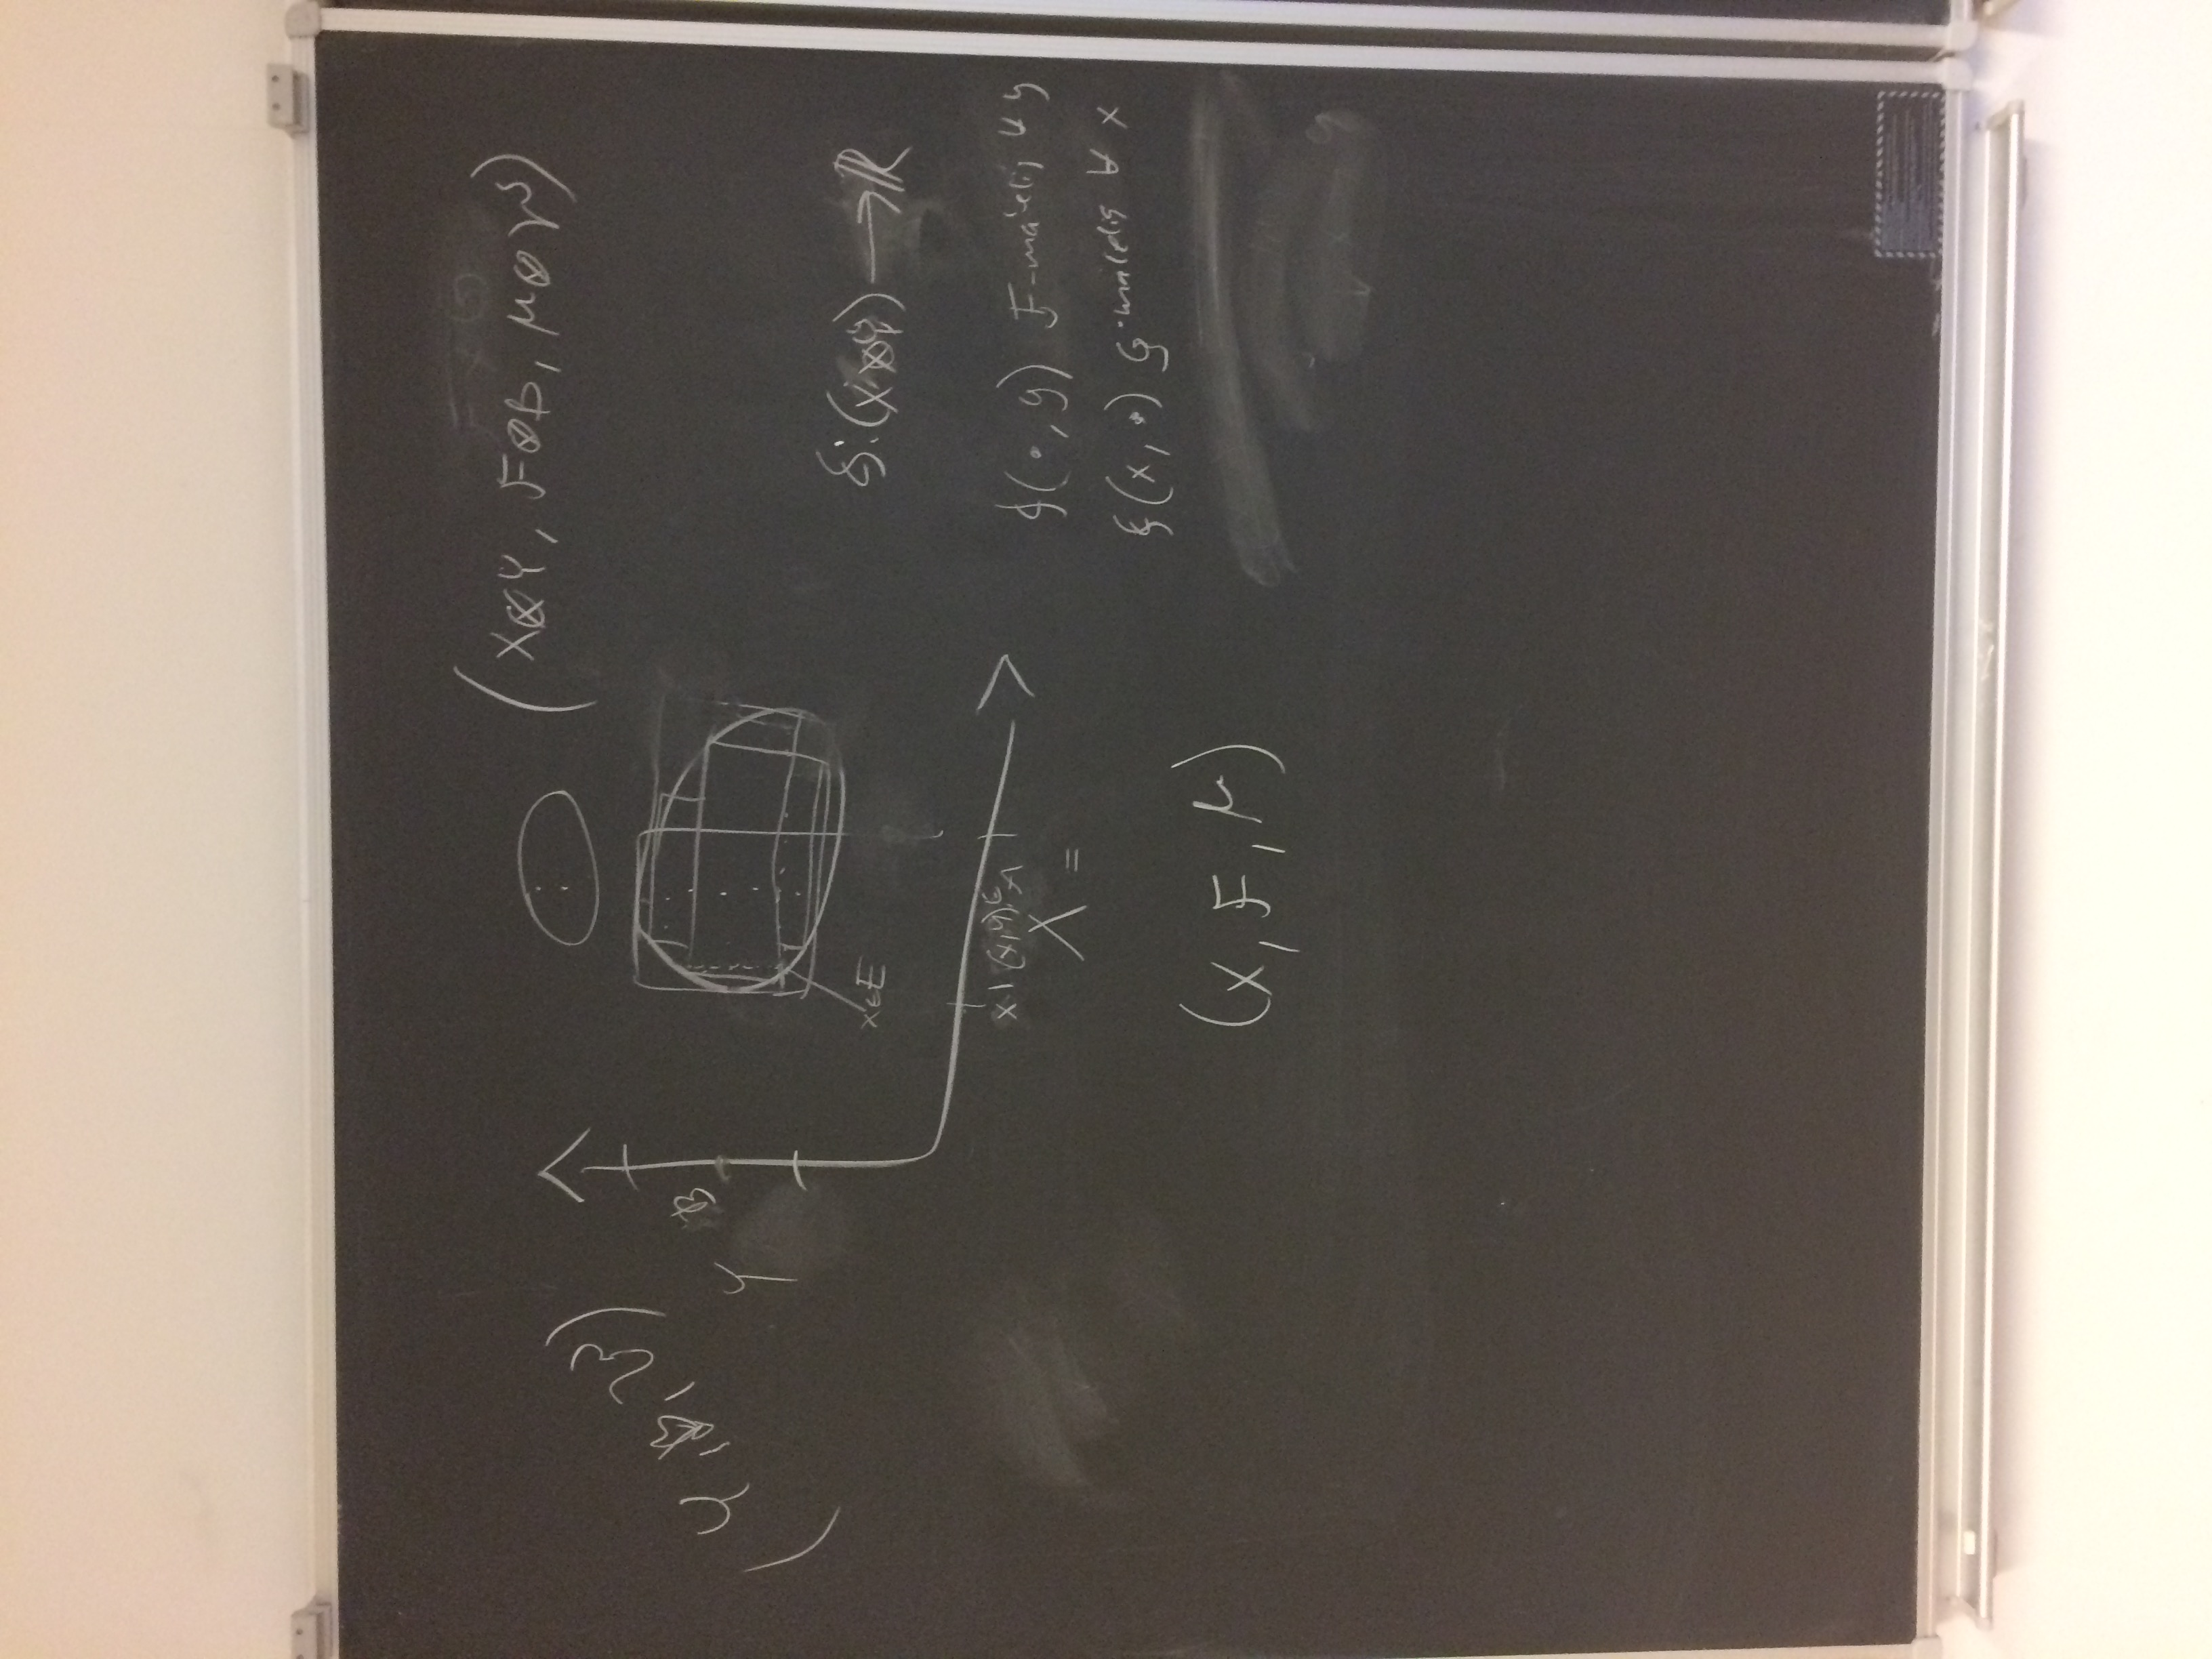
\includegraphics[scale=0.15,angle=270]{IMG_1}\captionof{figure}{\footnotesize Det kunne sikkert tegnes pænere.}\label{fig:prodspace}
\end{minipage}\\[0.7 em]

Så præsenteres \href{https://en.wikipedia.org/wiki/Pi_system}{$\pi$-systemer}, som er lukkede under fællesmængde og \href{https://en.wikipedia.org/wiki/Dynkin_system}{$\lambda$-systemer} som er lukkede under komplementærmængder og forening af disjunkte mængder, ydermere står der i mine noter at $\FI$, $\sigma$-algebra $\iff$ $\FI$ er et $\pi$-system og $\FI$ er et $\lambda$-system. 

\begin{theorem}[Dynkins $\pi$ - $\lambda$ sætning]\label{th:dynkin}
	Antag $\PI$ er et $\pi$-system og $\L$ er et $\lambda$-system. Hvis $\PI \subset \L$ så er $\sigma(\PI)\subset\L$
\end{theorem}
\begin{theorem}\label{th:s2}
	Hvis $E\in \FI \otimes \G$ så gælder for alle $y$ at $\{ x|(x,y)\in E \}\in \FI$ og for alle $x$ at $\{ y|(x,y)\in E \}\in \G$. Hvis $f$ er målelig $\FI \otimes \G$, så $f(x,\cdot)\in \G$ og $f(\cdot,y)\in \FI$. Se eventuelt figur \ref{fig:prodspace}
\end{theorem}
\begin{theorem}
	Der eksisterer et unikt mål $\lambda$ på $\{ X \times Y, \FI \otimes \G \}$ sådan, at
	\[ \lambda(A\times B)=\mu(A)\cdot\nu(B). \]
	for ethvert måleligt rektangel $A \times B$. Dette mål kaldes {\bf produktmål} og benævnes $\lambda=\mu\times\nu$.
\end{theorem}
\begin{proof}
	Dette er ikke et rigtigt bevis, men lidt derhenad. Vi viser kun for $\mu$ og $\nu$ endelige. Fra sætning \ref{th:s2} ses at $g_E(x)=\nu (\{ y|(x,y)\in E \})$ er en veldefineret funktion af $x$. Hvis $\L$ er klassen af de $E\in \FI \otimes \G$, som opfylder at $g_E(x)$ er målelig $\FI$ så er $\L$ et $\lambda$-system, som indeholder alle målelige rektangler (et $\pi$-system) og derfor ud fra sætning \ref*{th:dynkin} er lig med $\FI \otimes \G$. Derfor kan vi definere et mål $\pi'$
	\[ \pi'(E)=\int_X g_E(x)d\mu(x)=\int_X \nu(\{ y|(x,y)\in E \})d\mu(x) \]
	og med samme argumentation kan vi definere
	\[ \pi''(E)=\int_Y \mu(\{ x|(x,y)\in E \})d\nu(y). \]
	For målelige rektangler $A\times B$ ses det let, at
	\[ \pi'(A\times B) = \pi''(A\times B) = \mu(A)\nu(B). \]
	Hvis vi igen definerer $\L_0$ som klassen af alle $E$, hvor $\pi'(E) =\pi''(E)$, så har vi igen et $\lambda$-system som indeholder de målelige rektangler og som således indeholder $\FI \otimes \G$. Produktmålet er således defineret ved $\lambda(A)=\pi'(A)=\pi''(A)$.
\end{proof}
\begin{theorem}[Fubinis sætning]
	Betragt produktmålsrummet $\{ X\times Y, \FI \otimes \G,\mu \times \nu \}$ og lad $f\colon X\times Y\to \RR$ være en målelig afbildning. Antag enten at $f$ er integrabel over $X\times Y$ eller at $f$ er ikke negativ, så har vi at
	\[ \int_{X\times Y}fd(\mu \times \nu)=\int_X \left[ \int_Y f(x,y)d\nu(y) \right]d\mu(x)=\int_Y\left[ \int_X f(x,y)d\mu(x) \right]d\nu(y). \]
\end{theorem}
\begin{proof}
	Dette er helle rikke rigtigt et bevis. Hvis vi definerer $f(x,y)=I_{\{ (x,y)\in E \}}$, så ses det let at de to sidste udtryk i ligheden svarer til $\pi'(E)=\pi''(E)$, hvilket følger af ovenstående. Dernæst følger resultatet let for simple funktioner. For ikke negative funktioner $f$ følger resultatet ved at tilnærme $f$ med en voksende følge af simple funktioner og anvende monoton konvergens sætningen. For generelle $f$ følger resultatet ved standardopsplitning i $f^+$ og $f^-$.
	
	Resultatet i sætning \ref{th:s2} kan også udvides til at for ikke negative $f$ er
	\[ \int_Y f(x,y)d\mu, \int_Xf(x,y)d\nu \]
	målelige hhv mht $\FI$ og $\G$.
\end{proof}
\newpage
\section*{3. Radon Nikodyms sætning og ækvivalente sandsynlighedsmål.}
\begin{definition}
	Betragt et måleligt rum $(X,\FI)$, hvorpå der er defineret to seperate mål $\mu$ og $\nu$
	\begin{itemize}
		\item Hvis det for alle $A\in \FI$ holder, at
		\[ \mu(A)=0 \Rightarrow\nu(A)=0, \]
		så siges $\nu$ at være {\bf absolut konvergent} med hensyn til $\mu$ på $\FI$, benævnes $\nu \ll \mu$.
		\item Hvis det både gælder at $\mu \ll \nu$ og $\nu \ll \mu$, så siges $\mu$ og $\nu$ at være {\bf ækvivalente}, benævnes $\mu \sim \nu$.
		\item Hvis der eksisterer to udfald, $A$ og $B$ sådan at
		\begin{itemize}
			\item $A\cap B=\emptyset$
			\item $\mu(B)=0$, og $\nu(A)=0$.
		\end{itemize}
		Siges $\mu$ og $\nu$ at være gensidige {\bf singulære}, benævnes $\mu \perp \nu$.
		
	\end{itemize}
\end{definition}

\begin{theorem}[Radon-Nikodym sætningen]
	 Betragt et målrum $(X,\FI,\mu)$, hvor vi antager at $\mu$ er endeligt, altså at  $\mu(X)<\infty$. Antag et der eksisterer et mål $\nu$ på $(X,\FI)$ sådan at $\nu \ll \mu$ på $\FI$. Så eksisterer der en ikke negativ funktion $f\colon X\to \RR$ således at
	 \[ f \text{ er }\FI\text{-målelig.} \]
	 \[ \int_X f(x)d\mu(x)<\infty, \]
	 \[ \nu(A)=\int_A f(x)d\mu(x), \forall A\in \FI .\]
	 Funktionen $f$ kaldes den {\bf Radon-Nikodym afledte} af $\nu$ med hensyn til $\mu$. Den er unikt defineret $\mu$ næsten overalt, og skrives
	 \[ f(x)=\frac{d\nu(x)}{d\mu(x)}, \]
	 eller alternativt
	 \[ d\nu(x)=f(x)d\mu(x). \]
\end{theorem}
\begin{proof}
	Vi skitserer et bevis, og det er åbenbart \href{https://en.wikipedia.org/wiki/John_von_Neumann}{von Neumanns} skyld. Definer et nyt mål $\lambda$ ved at sætte $\lambda(A) = \mu(A)+\nu(A)$, for alle $A\in \FI$. For ethvert $g\in L^2(\lambda)$ kan vi definere en lineær afbildning $\Phi \colon X \to \RR$ ved
	\[ \Phi(g)=\int_Xg(x)d\nu(x), \]
	og fra trekant og Cauchy-Schwarz ulighederne har vi, at
	\begin{align*}
		|\Phi(g)|=\left\vert \int_X g(x)d\nu(x)\right\vert &\leq \int_X |g(x)|d\nu(x) \leq \int_X |g(x)|d\lambda(x)\\
		\int_X |g(x)|d\lambda(x)&\leq^{CS}\sqrt{\int_X\1 d\lambda(x)}\sqrt{\int_X g^2(x)d\lambda(x)}\\
		 &= \sqrt{\lambda(X)}\cdot ||g||_{L^2(\lambda)}. 
	\end{align*}
	Så har vi fra Reiz's repræsentationssætning at der eksisterer en $f\in L^2(\lambda)$ sådan at $\Phi(g)=(g,f)$ for alle $g\in L^2(\lambda)$, altså
	\begin{equation}
		\int_X g(x)d\nu(x)=\int_X g(x)f(x)d\lambda(x), \forall g\in L^2(\lambda).\label{eq:A14}
	\end{equation}
	Ved at vælge $g=I_A$ for et tilfældigt $A\in \FI$, har vi grundet $0\leq \nu(A)\leq\lambda(A)$, at $0\leq f \leq 1$. 
	\[ \int_X\1_A(x)d\nu(x)=\int_X f(x)\1_A(x)d\nu(x)\]
	\[ \nu(A)=\int_A f(x)d\lambda(x)=\int_A f(x)d\nu(x)+\int_A f(x)d\mu(x) \]
	\[ \nu(A)\geq \int_A f(x) d\nu(x) \Rightarrow f(x) \leq 1 \]
	
	Vi kan nu skrive ligning \ref{eq:A14} som
	\[ \int_Xg(x)d\nu(x)=\int_X g(x)f(x)d\nu(x)+\int_X g(x)f(x)d\mu(x), \]
	eller
	\[ \int_Xg(x)d\nu(x)-\int_X g(x)f(x)d\nu(x)=\int_X g(x)f(x)d\mu(x), \]
	\begin{equation}
		\int_X g(x)(1-f(x))d\nu(x)=\int_X g(x)f(x)d\mu(x), \forall g\in L^2(\lambda). \label{eq:A15}
	\end{equation}
	
	Lad $g$ være en indikatorfunktion
	\[ (1-f(x))d\nu=f(x)d\mu \]
	\[ \frac{1-f(x)}{f(x)}=\frac{d\mu}{d\nu} \]
	\[ \frac{d\nu}{d\mu}=\frac{f(x)}{1-f(x)}\]
\end{proof}
	\begin{comment}
	Da dette holder for alle $g\in L^2(\lambda)$ og i særdeleshed for alle indikatorfunktioner kan vi skrive dette på "differential form" (der refereres stil opgaverne, for at retfærdiggøre dette)
	\[ (1-f)d\nu=fd\mu. \]
	Det ville her være fristende at gange igennem med $(1-f)^{-1}$ for at få
	\[ d\nu=\frac{f}{1-f}d\mu, \]
	for så at definere den Radon-Nikodym afledte som $\frac{f}{(1-f)}$, men her kommer vi selvfølgelig i problemer når $f=1$. Definer derfor $A$ ved $A=\{ x\in X;f(x)=1 \}$, og sæt $g=I_A$. Så får vi fra \ref{eq:A15}, at
	\[ \int_A fd\mu=\int_A(1-f)d\nu=0, \]
	og da $f\geq 0$, er $\mu(A)=0$. Vi bruger nu antagelsen om at $\nu\ll\mu$ til at udlede at også $\nu(A)=0$, altså kan vi sagtens skrive
	\[ d\nu=\frac{f}{1-f}d\mu, \]
	og vi ser at den Radon-Nikodym afledede faktisk er givet ved
	\[ \frac{d\nu}{d\mu}=\frac{f}{1-f}.\]
\end{proof}

	content...

\begin{proof}[fra noter]
	 Antag $\mu,\nu$ er endelige (de skal egentligt være $\sigma$-endelige, men det viser vi ikke for)
	 Definer et nyt mål $\lambda\colon\lambda(A) = \mu(A)+\nu(A)$,  $g\in L^2(\lambda)$.
	 Definer $\Phi \colon L^2(\lambda) \to \RR$ sådan at
	\[ \Phi(g)=\int_Xg(x)d\nu(x), \]
	\begin{align*}
		|\Phi(g(x))|=&\left\vert \int_X g(x)d\nu(x)\right\vert \leq \int_X |g(x)|d\nu(x) \leq \int_X |g(x)|d\lambda(x)\\
		=&\int_X \sqrt{g(x)-1}^2d\lambda(x)\leq \sqrt{\int_X 1 d\lambda(x)}\sqrt{g^2(x)d\lambda(x)}\\
		=&\sqrt{\lambda(x)}\cdot ||g(x)||_{L^2(\lambda)}=K||g(x)||_{L^2(\lambda)}
	\end{align*}
	dermed er $\Phi$ en begrænset operator, så der findes en funktion $f$ så (grundet Riez's repræsentations sætning)
	\[ \Phi(g)= \langle f,g \rangle_{L^2(\lambda)}=\int_X fgd\lambda \]
	\[ \int_Xgd\mu=\int_X f\cdot g d\lambda \]
	
	
	$g=I_A$
	\[\int_A d\nu=\int_A fd\lambda = \int_A fd\nu+\int_A fd\mu \geq \int_A f d\nu \Rightarrow f\leq 1\]
	\begin{align*}
		&\int_X g d \nu=\int_Xfgd\nu+\int_Xfgd\mu\\
		\Rightarrow&\int_X g(1-f)d\nu=\int_Xfgd\mu\\
		\Rightarrow&\int_Xg(1-f)d\nu=\int_Xg(1-f)\frac{f}{1-f}d\mu\\
		\Rightarrow&\frac{d\nu}{d\mu}=\frac{f}{1-f}
	\end{align*}
	det fucker up når $f=1$
	
	$A=\{ x |f(x)=1 \}$
	\[ \int_A d\nu =\int_A f d \nu +\int_A fd\mu \]
	\[ \int_A 1-f d\nu=\int_A fd \mu \Rightarrow\int_A 0 d\nu = \int_A 1d\mu \Rightarrow0=\mu(A)\Rightarrow\nu(A)=0 \]
	da $\nu\ll\mu$
\end{proof}
Et lille eksempel:

	Det er vigtigt at forstå konceptet om at absolut kontinuitet er defineret relativt til en given $\sigma$-algebra. Hvis eksempelvis $\G \subseteq\FI$ kan det meget vel være at $\mu\ll\nu$ på $\G$ samtidig med, at det ikke holder at $\mu\ll\nu$ på $\FI$. Et trivielt eksempel gives ved at sætte $X=\{1,2,3\} $ og definere
	\[ \FI=2^X, \G=\{X,\emptyset,\{1\},\{2,3\}\} \]
	og
	\begin{align*}
		\mu(1)=&2, \mu(2)=&0, \mu(3)=&2\\
		\nu(1)=&8, \nu(2)=&5, \nu(3)=&13. 
	\end{align*}
	Her er det indlysende at vi IKKE har $\nu\ll\mu$ på $\FI$, da $\mu(2)=0$ samtidig med, at $\nu(2)\neq 0$. Vi har dog, at $\nu\ll\mu$ på $\G$, med Radon-Nikodym afledet givet ved
	\[f\left( x \right) = \left\{ \begin{gathered}
	4\hfill ~~for\,\, n=1 \\
	9\hfill ~~for\,\, n=2 \\
	9\hfill ~~for\,\, n=3 
	\end{gathered}  \right.\]
Bemærk i øvrigt at $f$ er $\G$-målelig.

Det ses at hvis vi udvider en $\sigma$-algebra kan vi miste den absolutte kontinuitet, men hvis  $\nu\ll\mu$ på et måleligt rum $(X,\FI)$ og $\G\subseteq\FI$, så gælder det også at $\nu\ll\mu$ på $\G$.

Så skal der med udgangspunkt i eksemplet forklares om ækvivalente sandsynlighedsmål, noget som er beskrevet i B6 side 500
\end{comment}


\newpage

\section*{4. Stokastiske variable og betingede middelværdier.}
%\subsection{Den endelige præsentation}
Givet et målrum \[(\Omega, \FI, P)\] definerer vi en stokastisk variabel ved den $\FI$-målelige funktion \[ X\colon\Omega \to  \RR,\] middelværdien af en sådan funktion betegnes \[ \EE\left[X\right]=\int_{\Omega} X(\omega)dP(\omega).\] Hvis en stokastiske variabel er betinget af et område $B$, begrænses integralet til $B$ og middelværdien normaliseres med sandsynligheden for at være i $B$, \[ \EE\left[X\vert B\right]=\frac{1}{P(B)}\int_{B} X(\omega)dP(\omega). \]
Vi betragter nu en opsplitning $\PI=\{A_1,A_2,...,A_n\}$ hvor $A_i$ og $A_j$ er disjunkte, når $i\neq j$. Derudover er $\bigcup\limits_{i=1}^{n} A_i=\Omega$. Middelværdien når der betinges med en opsplitning, kan ses som \[ \EE\left[X\vert \PI\right](\omega)=\sum\limits_{i=1}^{n} \EE\left[X\vert A_i\right]\1_{A_i}(\omega). \]
\begin{proposition}\label{prop:measurable_if_constant}
	Givet eg opsplitning $\PI$ og en stokastisk variabel $X\colon \Omega\to\RR$, siges $X$ at være $\sigma(\PI)$-målelig hviss $X$ er konstant på hvert komponent i $\PI$
\end{proposition}
Vi definerer nu \[ Z(\omega):=\sum\limits_{i=1}^{n} \EE\left[X\vert A_i\right]\1_{A_i}(\omega), \] hvor vi fra proporsition \ref{prop:measurable_if_constant} har at $Z$ er $\sigma(\PI)$-målelig. Lad $G\in \sigma(\PI)$, så har vi at
\begin{align*}
	\int_G ZdP&=\int_G\sum\limits_{i=1}^{n} \EE\left[X\vert A_i\right]\1_{A_i}dP \\
	&=\int_\Omega\sum\limits_{i=1}^{n} \1_G\EE\left[X\vert A_i\cap G\right]\1_{A_i}dP\\
	&=\sum\limits_{i=1}^{n} \int_\Omega \1_G\EE\left[X\vert A_i\cap G\right]\1_{A_i}dP\\
	&=\sum\limits_{i=1}^{n} \int_\Omega \EE\left[X\vert A_i\cap G\right]\1_{A_i\cap G}dP\\
	&=\sum\limits_{i=1}^{n} \EE\left[X\vert A_i\cap G\right]\int_\Omega \1_{A_i\cap G}dP\\
	&=\sum\limits_{i=1}^{n} \EE\left[X\vert A_i\cap G\right]P(A_i\cap G)\\
	&=\sum\limits_{i=1}^{n} \frac{1}{P(A_i\cap G)} \int\limits_{A_i\cap G}XdP~~ P(A_i\cap G)\\
	&=\sum\limits_{i=1}^{n} \int\limits_{A_i\cap G}XdP=\int_G X dP\\
\end{align*}
$\EE\left[ X\vert \G\right]$ defineres til at være den stokastiske variabel $Z$, som opfylder at $Z$ er målelig $\G$ og $\int_G ZdP=\int_G X dP$ for alle $G\in\G$.
\begin{theorem}
	Denne eksisterer altid og er unik!
\end{theorem}
\begin{proof}
	Definer $\nu(G)=\int_G X(\omega)dP(\omega)$ på $(\Omega,\G)$ og antag $x\geq0$. Da er $\nu \ll P$, eftersom $P(A)=0\Rightarrow \nu(A)=0$. Så benyttes Radon-Nikodym: Definer $Z$ på $\G$ sådan at \[ Z=\frac{d\nu}{dP}\iff d\nu =ZdP \] som vi ved eksisterer fra Radon-Nikodym. Da er \[ \int_G Z dP = \int_G d\nu = \nu(G) = \int_G X dP, \forall G\in\G\] da Radon-Nikodym  siger at den afledede er entydig.
\end{proof}
%\subsection{Tidligere noter, med forbehold for fejl, burde udkommenteres}
%Det vi kunne tænke os er en brugbar definition af objektet
%\[ \EE[X|\G], \]
%hvor $X$ er en stokastisk variabel og $\G$ er en 	$\sigma$-algebra inkluderet i $\FI$. Fortolkningen skulle gerne være, at $\EE[X|\G]$ er "forventningen (middelværdien) af $X$ givet at vi har adgang til informationen i $\G$". Det er ikke trivielt at formalisere denne let flygtige beskrivelse, så vi starter med en logisk tankerække.
%
%Vi starter med den ubetingede middelværdi givet ved
%\[ \EE[X]=\int_{\Omega}X(\omega)P(d\omega), \]
%altså er $\EE[X]$ et vægtet gennemsnit af værdier af $X$, hvor vi har brugt sandsynlighederne $P(d\omega)$ som vægte.
%
%Antag nu at vi har skaffet oplysninger om det stokastiske eksperiment, i det omfang at vi ved, at stikprøven $\omega$ ligger i mængden $B$. Den naturlige definition af den forventede værdi af $X$ givet $B$ findes nu gennem det vægtede gennemsnit af $X$ over det nye effektive udfaldsrum $B$. Vi skal selvfølgelig normalisere sandsynlighedsmålet så vi har total masse lig med forening på det nye rum $B$. Derfor normaliserer vi sandsynlighederne som 
%\[ \frac{P(d\omega)}{P(B)}, \]
%og vi kan nu definere objektet $\EE[X|B]$.
%\begin{definition}
%	Antag $B\in \FI$ med $P(B)>0$, og at $X\in L^1(\Omega,\FI,P)$. Så er "den betingede middelværdi af $X$ givet $B$"  defineret ved
%	\[ \EE[X|B]=\frac{1}{P(B)}\int_B X(\omega)dP(\omega).\]
%\end{definition}
%\begin{theorem}
%	Det er jeg ikke helt sikker på...
%\end{theorem}
%\begin{proof}
%	content...
%\end{proof}
\newpage

\section*{5. Martingaler og stoppetider.}
\begin{definition}[Filtrering]
	Givet et sandsynlighedsrum $(\Omega, \FI, P)$ er en \textbf{filtrering} en indekseret følge af $\sigma$-algebraer $\left\{ \FI_t \right\}_{t\geq 0}$,  benævnes $\FIU$, hvorom det gælder:
	\begin{enumerate}
		\item $\FI_t \in \FI \forall t$
		\item $s<t \Rightarrow \FI_s^X\subset \FI_t^X$
	\end{enumerate}
	Med en sådan filtrering har vi et filtreret sandsynlighedsrum $(\Omega, \FI, P,\FIU)$
\end{definition}

\begin{definition}[Tilpasset]
	$X$ er \textbf{$\FIU$-tilpasset} hvis $X_t\in\FI_t$
\end{definition}

\begin{definition}[Martingale]
	Givet et filtreret sandsynlighedsrum $(\Omega, \FI, P,\FIU)$ er den stokastiske process $X$ et \textbf{martingale} hvis:
	\begin{enumerate}
		\item $X$ er $\FIU$-telpassr
		\item $X_t\in L^1 \forall t$
		\item $\forall s \& t$ når $0\leq s \leq t$ er $X_s=\EE[X_t\vert \FI_s]$, $P$ n.s.
	\end{enumerate}
\end{definition}

\begin{definition}[Kvadratintegrabelt martingale]
	Hvis $\EE \left[ X_t^2 \right]\leq M \forall t,t\in[ 0,\infty [$, siges $X$ at værre \textbf{kvadratintegrabel}
\end{definition}
\begin{theorem}[Martingal konvergens]
	Antag $X$ er kvadratintegrabel, så eksisterer $X_\infty$ hvorom det gælder, at $X_t\to X_\infty$ i $L^2$ og $P$ n.o., når $t\to \infty$.
	Ydermere gælder det at $X_t=\EE[ X_\infty\vert\FI_t ]\forall t\geq 0$.
\end{theorem}

\begin{definition}[Stoppetid]
	Givet et filtreret sandsynlighedsrum $(\Omega, \FI, P, \FIU)$, er en \textbf{stoppetid} med hensyn til filtreringen $\FIU$ en ikke negativ stokastisk variabel $T$ således at
	\[ \{T\leq t\}\in\FI_t, \text{ for ethvert }t\geq 0.\]
\end{definition}
\begin{theorem}[Optional Sampling Theorem]
	Antag at $X$ er en martingal som opfylder
	\[ \sup\limits_{t\geq 0}\EE\left[ X_t^2 \right] \leq \infty.\]
	Lad $S$ og $T$ være stoppetider hvor $S\leq T$, så gælder det at
	\[ \EE\left[ X_T\vert \FI_S \right]=X_S, ~~ P \text{  n.s.} \]
	%Hvis $X$ er en submartingale som opfylder samme integrabilitetsbetingelse, så holder resultatet med $\geq$ i stedet for $=$.
\end{theorem}
\begin{proof}
	Vi begrænser os til diskret tid. Fra martingal konvergens sætningen har vi at der eksisterer en stokastisk variabel $Y$ sådan at 
	\begin{equation}\label{eq:C.16}
		X_n=\EE\left[ Y\vert \FI_n \right], ~~n=0,1,...
	\end{equation}
	Det er så åbenbart nok HVORFOR? (tak for lort bog) at vise, at for en hvilken som helst stoppetid $T$ har vi
	\[ \EE\left[ Y\vert \FI_T \right]=X_T \]
	altså skal vi vise, at for alle $A\in\FI_T$ har vi 
	\[ \int_{A} Y dP=\int_A X_T dP. \]
	Ved at skrive $A$ som $A=\bigcup_n(A\cap\{T=n\})$, husker vi at $A\cap\{T=n\}\in \FI_n$, og bruger ligning \ref{eq:C.16} får vi
	\[ \int_A YdP=\sum\limits_{n=0}^{\infty}\int_{A\cap \{T=n\}} YdP= \sum\limits_{n=0}^{\infty}\int_{A\cap \{T=n\}} X_n dP= \int_A X_T dP.\]
\end{proof}
\newpage

\section*{6. Brownske bevægelser og stokastiske integraler.}
\begin{definition}[Wienerprocess]
	En wienerprocess $W$ er en stokastisk process som opfylder, at:
	\begin{enumerate}
		\item $W(0)=0$
		\item Uafhængige intervaller: $r<s\leq t < u\Rightarrow W(u)-W(t) \& W(s)-W(r)$ er uafhængige stokastiske variable.
		\item For $s<t \Rightarrow W(t)-W(s)\sim N(0,\sigma), \sigma=\sqrt{(t-s)}$
		\item $W$ har kontinuerte spor/baner
	\end{enumerate}
\end{definition}
Givet klassen $\pounds^2[a,b]$, ligger $g$ i $\pounds^2$ hvis:
\begin{enumerate}
	\item $\int_{a}^{b}\EE\left[g^2(s)\right]ds<\infty$
	\item $g$ er $\FI_tW$- tilpasset
\end{enumerate}
Gvet klassen $\pounds^2[a,b]$ ligger $g$ i $L^2$ hvis:
\begin{itemize}
	\item $g$ ligger i  $\pounds^2[0,t],~ \forall t$
\end{itemize}
\begin{definition}[Stokastisk integrale]
	Det stokastiske integrale for en simpel funktion g(s) er givet ved
	\[ \int_a^b g(s) ds =\sum\limits_{k=0}^{n-1}g(t_k)[W(t_{k+1})-W(t_k)],~a=t_0,b=t_n,~t_0<t_1<...<t_n \]
\end{definition}
For et generelt $g_n(s)$ \[ \int_{a}^{b}\EE\left[ g_n(s)-g(s) \right]^2ds \xrightarrow{n\to\infty} 0 \] og \[ \int_{a}^{b} g(s) ds= \lim\limits_{n\to \infty}\int_{a}^{b} g_n(s) ds\]
\begin{theorem}
	Lad $g$ ligge i $\pounds^2$ så har vi:
	\begin{enumerate}
		\item $\EE\left[\int_{a}^{b} g(s) dWt  \right]=0$
		\item $\EE\left[\left(\int_{a}^{b} g(s) dWt\right)^2  \right]=\int_{a}^{b}\EE\left[g^2(s)   \right]dWt$
		\item $\int_{a}^{b} g(s) dWt  $ er $\FI_b^W$-måleligt
	\end{enumerate}
\end{theorem}
\begin{proof}
	Det er ikke sådan ligetil, så vi nøjes med at vise "1" for en simpel funktion.
	\[ \EE\left[\int_{a}^{b} g(s) dWt  \right]=\EE\left[ \sum\limits_{k=0}^{n-1}g(t_k)\Big(W(t_{k+1})-W(t_k)\Big)\right] \]
	da middelværdier er lineære
	\[ =\sum\limits_{k=0}^{n-1}\EE\left[ g(t_k)\Big(W(t_{k+1})-W(t_k)\Big)\right] \]
	da $g$ er tilpasset afhænger $g$ af $t_k$ kun gennem wienerproces på $[0,t_n]$
	\[ =\sum\limits_{k=0}^{n-1}\EE\left[ g(t_k)\right] \EE\left[(W(t_{k+1})-W(t_k)\right]\]
	fra definitionen af wienerprocesser ved vi at middelværdien af tilvæksten er $0$ og når man ganger med $0$ er det hele
	\[=0\]
\end{proof}
\newpage

\section*{7. Stokastiske differentialligninger, diffusioner og Itos formel.}
\begin{definition}[Diffusionsproces]
	En diffusionsproces $\{X_t\}$ er givet ved følgende: $\{h(s) \}$, $\{ g(s) \}$ to stokastiske processer, $h,g\in \pounds^2$ og $h,g$ er tilpasset $\FI_t^\omega$ \[ X(t)-X(0)=\int_0^t h(s)ds+\int_0^t g(s) dW(s), \] hvor udtrykket før $+$ er driftled og udtrykket efter er diffusionsled.
	\[ \EE\left[  X(t)-X(0) \right] = \int_0^t \EE\left[h(s)\right] ds+\EE\left[\int_0^t g(s) dW(s)\right]\]
	Da middelværdien af diffusionsledet altid er $0$ gælder det at: $\{X_t\}$ er en martingale hvis og kun hvis $h(s)=0\forall s$.
\end{definition}
\begin{definition}[Stokastisk differentialligning]
	Las $\mu$ og $\sigma$
\end{definition}
\begin{theorem}[Itôs formel]
	Givet et  filtreret sandsynlighedsrum $(\Omega, \FI, P, \FIU)$, en Wienerproces $W(s)$ med hensyn til $\FI$, to processer $\mu(s)$ og $\sigma(s)$ tilpasset $\FIU$ og $\mu(s),\sigma(s) \in \pounds^2$ er \[ dZ(t)=\left( f_t(t,X(t))+\mu(t)f_X(t,X(t))+\frac{1}{2}\sigma(t)f_{XX}(t,X(t)) \right)dt+\sigma(t)f_X(t,X(t))dW(t) \]
	
\end{theorem}
Her mangler jeg bestemt noget forklaring om hvad der er hvad. Hvorefter vi forklarer hvad et stokastisk differentiale er, ud fra en geometrisk Brownsk bevægelse \[ dX(t)=\alpha X(t) dt +\sigma X(t) dW(t),\]
\[X(0)=x. \]
Vi ønsker så at løse denne differentialligning med Itôs formel, og starter med $ln(X)$, som giver mening da $\frac{\frac{dX}{dt}}{X(t)}=\alpha$
\[ Z(t)=ln(X(t))=f(X(t)), \] vi skal bruge nogle afledte $f_t=0, f_X=\frac{1}{X}, f_{XX}=-\frac{1}{X^2}$ og indsætter i Itôs formel
\begin{align*}
	dZ(t)&=\frac{1}{X(t)}\left( \alpha X(t) +\sigma X(t) dW(t) \right)-\frac{1}{2}\frac{1}{X^2(t)}\sigma^2X^2(t)dt\\
	&=\left(\alpha-\frac{1}{2}\sigma^2\right)dt+\sigma dW(t)
\end{align*}
Vi trækker nu $Z(0)$ fra $Z(t)$
\begin{align*}
	Z(t)-Z(0)&=\int_{0}^{t}\alpha-\frac{1}{2}\sigma^2ds+\int_{0}^{t}\sigma dW(s)\\
	&=\left( \alpha-\frac{1}{2}\sigma^2 \right)t+\sigma W(t)
\end{align*}
da $e^{Z(t)-Z(0)}=e^{\left(\alpha - \frac{1}{2}\sigma^2\right)t+W(t)}$ og $\frac{X(t)}{x}=e^{\left(\alpha-\frac{1}{2}\right)t+\sigma W(t)}$ har vi at 
\[ X(t)=xe^{\left(\alpha-\frac{1}{2}\sigma^2\right)t+\sigma W(t)} \]
Vi søger nu middelværdien
\begin{align*}
	\EE\left[X(t)\right]&=\EE\left[ xe^{\left(\alpha-\frac{1}{2}\sigma^2\right)t+\sigma W(t)} \right]\\
	&=xe^{\left(\alpha-\frac{1}{2}\sigma^2\right)t}\EE\left[ e^{\sigma W(t)} \right]
\end{align*}
og nu bliver det spændende, for jeg er ikke helt sikker på rækkefølgen af mine noter, men det er noget med at man ikke sådan bare lige finder den der middelværdi til sidst, så derfor husker vi at $X(t)$ er en geometrisk Brownsk bevægelse, siger
\begin{align*}
	m(t)=\EE[X(t)]\\
	m'(t)=fm(t)\\
	m(t)=ce^{\alpha t}\\
	m(0)=c-x\\
	m(t)=xe^{\alpha t}\\
	\EE\left[ e^{\sigma W(t)} \right]=e^{\frac{1}{2}\sigma^2 t}
\end{align*}
hvorefter eller inden vi husker den anden måde at skrive en differentialligning på
\[ X(t)=\alpha +\int_{0}^{t}\alpha X(t) dt+ \int_{0}^{t}\alpha  X(t)dW(t)\]
\[ \EE\left[ X(t) \right]=x+\int_{0}^{t}\alpha\EE\left[ X(t) \right]dt+0. \]
Så $dX(t)=aX(t)dt+\sigma dW(t)$ så har jeg skrevet "integrating factor" og jeg ved ikke helt hvorfor, $Z(t)=e^{kt}X(t)-f(t,x)$. $f_t=ke^{kt}x, f_x=e^{kt},f_{xx}=0$ så er der lige en differentialligning igen, man kunne tro, at vi er igang med endnu en omgang Itô
\[ dZ(t)=ke^{kt}X(t)dt+e^{kt}aX(t)dt+\frac{1}{2}\sigma^2 0dt+e^{kt}\sigma dW(t) \]
\[ dZ(t)=(k+a)Z(t)dt+e^{kt}\sigma dW(t) \]
\[ k=-a\Rightarrow dZ(t)=e^{-at}\sigma dW(t) \]
\[ Z(t)-Z(0)=\sigma\int_{0}^{t}e^{-as}dW(s)\Rightarrow e^{-at}(X(t)-X(0)) = \sigma\int_{0}^{t}e^{-as}dW(s) \]
\[ X(t)-X(0)=\sigma\int_{0}^{t}e^{a(t-s)}dW(s) \]

\newpage

\section*{8. Girsanovs Sætning.}

\begin{theorem}[Girsanovs Sætning]
	Betragt det filtrerede målrum $(\Omega ,\FI,P,\FIU)$, og intervallet $[0,T]$. Lad $W^P=\left\{ W^P_{(t)} \right\}$ være en wienerproces med hensyn til $(P,\FI)$. Lad $\left\{ \phi_{(s)} \right\}$ være $\FI$-tilpasset. Definer$L=\{ L(t) \}$ ved:
	\begin{enumerate}[label=(\alph*)]
		\item \[dL(t)=L(t)\phi(t)dW^P(t)\] \[ LW=1 \] Vi antager $\EE[L(t)]=1.$ Så definerer vi mål $\Q$ på $\FI_T$ da $d\Q =L_T dP$ så gælder at
		\item $d W^P(t)=\phi(t)dt +dW^\Q(t)$, hvor $\{W^\Q(t)\}$ er en wienerproces med hensyn til $(\Q,\FI_T)$
	\end{enumerate}
\end{theorem}
\begin{proof}
	Vi skal vise at under $\Q$ har vi 
	\begin{enumerate}
		\item $W^\Q(0)=0$
		\item $W^\Q(t)-W^\Q(s)\perp\FI_s$ for alle $s<t$
		\item $W^\Q(t)-W^\Q(s)\sim N(0,t-s)$ for alle $s<t$ for alle $t$
	\end{enumerate}
	$W^\Q(0)=0$ vælges. Hvis vi viser at $\EE^\Q[e^{iu(W^\Q(t)-W^\Q(s)}\vert \FI_s]=e^{-\frac{1}{2}u(t-s)}$ er vi hjemme (med Bjarnes ord).
	Vi sætter $(s=0)$ så $\EE^\Q[e^{iuW^\Q(t)}]=\EE^P[L_te^{iuW^\Q(t)}]$. Med Ito's formel ($f(x,y)=xy, f_x=y,f_y=x,f_{xy}=f_{yx}=1$)
	\[ d\left(L_t e^{iuW^\Q(t)}\right)=dL_t e^{iuW^\Q(t)}+L_td\left( e^{iuW^\Q(t)} \right)+dL_t\left( de^{iuW^\Q(t)} \right) \]
	\[ d\left( e^{iuW^\Q(t)} \right)=iue^{iuW^\Q(t)}dW^\Q(t)+\frac{1}{2}\left(-u^2\right)e^{iuW^\Q(t)}\left(dW^\Q(t)\right)^2 \]
	\begin{align*}
		d\left( L_t e^{iuW^\Q(t)} \right)&=e^{iuW^\Q(t)}\Bigg( L(t)\phi(t)dW^P(t)+L(t)\left( iudW^\Q(t)-\frac{u^2}{2}dt  \right)\\		  
		&+\left( L(t)\phi(t)dW^P(t) \right)\left( iudW^\Q(t)-\frac{u^2}{2}dt \right)\Bigg)\\
		&=e^{iuW^\Q(t)} L(t) \Bigg( \phi(t)dW^P(t) + iudW^\Q(t)-\frac{u^2}{2}dt\\
		&+\phi(t)dW^P(t)\left(iudW^\Q(t)-\frac{u^2}{2}dt\right)\Bigg)\\
		&=e^{iuW^\Q(t)}L(t)\left( \phi(t)dW^P(t)+iudW^\Q(t)-\frac{u^2}{2}dt+iu\phi(t)dt \right)
	\end{align*}
	Altså er \[ z(t)=e^{iuW^\Q(t)}L(t) \]
	og
	\begin{align*}
		dz(t)&=z(t)\left( \phi(t)dW^P(t)+iudW^P(t)-iu\phi(t)dt-\frac{u^2}{2}dt+iu\phi(t)dt\right)\\
		&=z(t)\left( -\frac{u^2}{2}dt+\left( \phi(t)+iu \right)dW^P(t) \right)
	\end{align*}
	Så\[ z(t)-z(0)=\int_{0}^{t}-z(s)\frac{u^2}{2}ds+\int_{0}^{t}z(s)\left( \phi(s)+u \right)dW^P(s) \]
	\[ \phi^\Q(u)=\EE^P[z(t)]=m(t) \]
	\[\EE[z(t)]-z(0)=-\int_{0}^{t}\EE(z(s))\frac{u^2}{2}ds+\EE\int_{0}^{t}z(s)(\phi(s)+u)dW^P(s)\]
	\[m(t)=1-\int_{0}^{t}m(s)\frac{u^2}{2}ds\]
	\[ m(t)=e^{-\frac{u^2}{2}t} \]
	Vi vil nu vise, at
	$\EE\left[e^{iu(W^\Q(t)-W^\Q(s))}\vert\FI_s\right] =e^{-\frac{1}{2}u^2(t-s)}$ for $A\in \FI_s$
	\begin{align*}
		\int_A \EE\left[  e^{iu(W^\Q(t)-W^\Q(s))}\vert\FI_s\right]d\Q&=\int_A e^{-\frac{1}{2}u^2(t-s)}d\Q\\
		\EE^\Q\left[ \1[A]e^{iu(W^\Q(T)-W^\Q(s))} \right]&=e^{-\frac{1}{2}u^2(t-s}\Q A\\
		\EE^P\left[ \1[A]L_t e^{u(W^\Q(T)-W^\Q(s))} \right]&=e^{-\frac{1}{2}u^2(t-s}\Q A
	\end{align*}
	Vi ser nu at\[ z(t)=\1[A]e^{-iuW^\Q(s)}L(t)e^{iuW^\Q(t)} \]
	og $dz(t)=\1[A]e^{-iuW^\Q(s)}d\tilde{z}(t)$ hvor $d\tilde{z}(t)$ er $z(t)$ fra før. Altså er $z(s)=L(s)\1[A]$ og $z(t)=z(s)$ hvilket giver os at
	\[ z(t)=z(s)\left( e^{-\frac{u^2}{2}(t-s)-\frac{1}{2}\int_{s}^{t}(iu+\phi(v))^2dv+\int_{s}^{t}(iu+\phi(v))dW^P(v)} \right) \]
	Så
	\begin{align*}
		\EE[z(t)]&=\EE^P\left[ z(s)e^{-\frac{u^2}{2}} \right]\\
		&= \EE^P\left[ L(s)\1[A]e^{-\frac{u^2}{2}} \right]\\
		&= \EE^\Q\left[ \1[A]e^{-\frac{u^2}{2}} \right]\\
		&=e^{-\frac{u^2}{2}}\Q A
	\end{align*}

\end{proof}



\end{document}